\setcounter{chapter}{7-1}

\chapter{Neural Networks 2 - Back-Propagation and Training}


\setcounter{section}{4}
%\pagebreak
%%%%%%%%%%%%%%%%%%%%%%%%%%%%%%%%%%%%%%%%%%%%%%%%%%%%%%%%%%%%%%%%%%%%%%%%%%%%%  
\section{Error back-propagation }

    We have a complete neural network: a \textbf{model} we can use to make predictions or calculations.
    
    Now, our mission is to \textbf{improve} this neural network: even if our hypothesis class is good, we still have to \textbf{find} the hypotheses that are useful for our problem.
    
    As usual, we will start out with \textbf{randomized} values for our weights and biases: this \textbf{initial} neural network will not be useful for anything in particular, but that's why we need to improve it.
        \note{We randomize them because otherwise, if our initialization is \\$w_i=0$, we get $$w^T x+w_0=0$$ no matter what input $x$ we have.}
    
    For such a complex problem, we definitely can't find an explicit solution, like we did for ridge regression. Instead, we will have to rely on \textbf{gradient descent}.\\
    
    \begin{concept}
        \vocab{Neural networks} are typically optimized using \purp{gradient descent}.
    \end{concept}
    
    \phantom{}
    
    \subsection{Review: Gradient Descent}
    
        What does it really mean to do gradient descent on our \textbf{network}? Let's remind ourselves of how gradient descent works, and then \textbf{build} up to a network.
        
        \begin{concept}
            \vocab{Gradient descent} works based on the following reasoning:
        
            \begin{itemize}
                \item We have a function we want to \purp{minimize}: our loss function $\loss$, which tells us how \gren{badly} we're doing.
                    
                \item We want to perform "less badly". Our main tool for \purp{improving} $\loss$ is to alter $\theta$ and $\theta_0$.
                    \begin{itemize}
                        \item These are our \gren{parameters}: we're adjusting our model.
                    \end{itemize}

                    
                \phantom{}
                
                    
                \item The \purp{gradient} is our main tool: $\pderiv{B}{A}$ tells you the direction to \gren{change} $A$ in order to \redd{increase} $B$.
                
                \item We want to \gren{change} $\theta$ to \redd{decrease} $\loss$. Thus, we move in the direction of 
                    
                    \begin{equation*}
                        \Delta \theta = -\eta \pderiv{\loss}{\theta}
                    \end{equation*}
                    
                \item We take steps $\Delta \theta$ (and $\Delta \theta_0$) until we are satisfied with $\loss$, or it \gren{stops} improving.
            \end{itemize}
            
        \end{concept}

            \note{Remember that $\eta$ is our \vocab{step size}: we can take bigger or smaller steps in each direction.}
        
    \phantom{}  
        
    \subsection{Review: Gradient Descent with LLCs}
    
        Let's start with a familiar example: \textbf{LLCs}.
        
        Our LLC model uses the following equations:
            \note{We'll use $w$ instead of $\theta$.}
        
        \begin{equation}
            \red{
                z(x) = w^T x + w_0  
            }
            \qquad \qquad
            \blu{
                g(z) = \sigma(z) = \frac{1}{1+e^{-z}}
            }
        \end{equation}
        
        \begin{equation}
            \pur{
                \loss(g,y) = y\log(g) + (1-y)\log(1-g)
            }
        \end{equation}
        
        Our goal is to minimize $\loss$ by adjusting $\theta$ and $\theta_0$.
        
        So, we want 
        
        \begin{equation}
            \pderiv {\pur{\loss}} {w} 
            \qquad \text{and} \qquad 
            \pderiv {\pur{\loss}} {w_0}
        \end{equation}
        
        We did this by using the \textbf{chain rule}:
            \note{We'll focus on $w$, but the same goes for $w_0$.}
        
        \begin{equation}
            \pderiv {\pur{\loss}} {w} 
            =
                \overbrace{
                \pderiv {\pur{\loss}} {\blu{g}} 
                    \cmul
                \pderiv {\blu{g}}     {w}
            }^{\loss(g)}
        \end{equation}
        
        We can break it up further using \textbf{repeated} chain rules:
        
        \begin{equation}
            \pderiv {\pur{\loss}} {w} 
            =%Goal: overlapping braces.
            \mathrlap{ %\mathrlap allows brace to overlap with the next section
                \overbrace{ %Create brace
                    \phantom{ %Create phantom text so our brace is the right size
                        \pderiv {\pur{\loss}} {\blu{g}} 
                            \cmul
                        \pderiv {\blu{g}}     {\red{z}}
                    }
                }^{\loss(g)} %Brace superscript
            }
            \pderiv {\pur{\loss}} {\blu{g}} 
                \cmul
            \underbrace{
                \pderiv {\blu{g}}     {\red{z}}
                    \cmul
                \pderiv {\red{z}}     {w}
            }_{g(z)}
        \end{equation}
        
        Plugging in our derivatives, we get:
        
        \begin{equation}
            \pderiv {\pur{\loss}} {w}
            =
            \overbrace{
                -
                \Big(
                    \frac{ \org{y} } { \blu{\sigma} } 
                    -
                    \frac{ 1-\org{y} } { 1 - \blu{\sigma} }
                \Big)
            }^{ \pderivslash{\loss}{g} }
            \cdot
            \overbrace{
                \blu{\sigma} (1-\blu{\sigma})
            }^{ \pderivslash{g}{z} }
            \cdot 
            \overbrace{
            x
            }^{ \pderivslash{z}{w} }
        \end{equation}

        \begin{concept}
            The \vocab{chain rule} allows us to take the gradient of \purp{nested functions}, where each function is the \gren{input} to the next one.
            
            Another way to say this is that one function \vocab{feeds into} the next.
        \end{concept}
            
            \note{If you aren't familiar with "nested" functions, consider this example:\\
            \phantom{ }\\
            If you have functions $f(x)$ and $g(x)$, then $g(f(x))$ is the \textbf{nested} combination, where the output of $f$ is the input of $g$.}
    
    \phantom{}
    
    \subsection{Review: LLC as Neuron}
    
        Remember that we can represent our LLC as a \textbf{neuron}: this could give us the first idea for how to train our \textbf{neural network}!
        
        \begin{figure}[H]
            \centering
            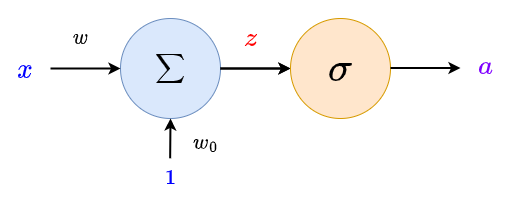
\includegraphics[width=80mm,scale=0.4]{images/nn_2_images/llc_as_neuron.png}
        \end{figure}
        
        As usual, our first unit $\sum$ is our \textbf{linear} component. The output is $z$, nothing different from before with LLC.
            \note{Remember that $x$ is a whole vector of values, which we've condensed into one variable.}
        
        The \textbf{output} of $\sigma$, which we wrote before as $g$, is now $a$.
        
        Something we neglected before: this diagram is \textbf{missing} the \textbf{loss function}. Let's create a small unit for that. 
        
        $\loss(a,y)$ has \textbf{two} inputs: our predicted value $a$, and the correct value $y$. 
        
        \begin{figure}[H]
            \centering
            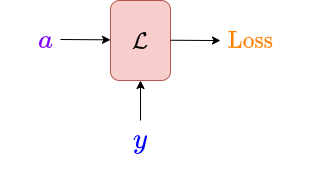
\includegraphics[width=60mm,scale=0.4]{images/nn_2_images/loss_unit.png}
            \caption*{We have two inputs to our loss function.}
        \end{figure}
        
        We \textbf{combine} these into a single unit to get:
        
        \begin{figure}[H]
            \centering
            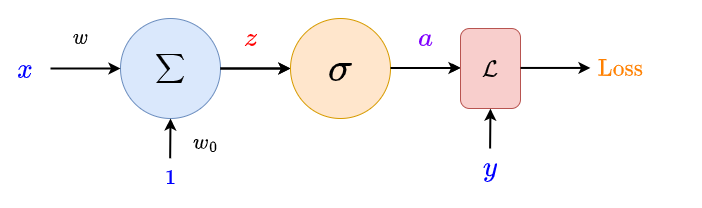
\includegraphics[width=90mm,scale=0.4]{images/nn_2_images/llc_as_neuron_loss.png}
        \end{figure}
        
        Our full unit!
        
    \phantom{}
    
    \subsection{LLC Forward-Pass}
    
        Now, we can do gradient descent like before. We want to get the effect our \textbf{weight} has on our \textbf{loss}.
        
        But, this time, we'll pair it with a \textbf{visual} that is helpful for understanding how we \textbf{train} neural networks. 
        
        First, one important consideration:
        
        As we saw above, the \textbf{gradient} we get might rely on $z$, $a$, or $\loss(a,y)$. So, before we do anything, we have to \textbf{compute} these values.
        
        Each step \textbf{depends} on the last: this is what the \textbf{forward} arrows represent. We call this a \textbf{forward pass} on our neural network.\\
        
        \begin{definition}
            A \vocab{forward pass} of a neural network is the process of sending information "\gren{forward}" through the neural network, starting from the \purp{input}.
            
            This means the \purp{input} is fed into the \gren{first} layer, and that output is fed into the \gren{next} layer, and so on, until we reach our \purp{final} result and \purp{loss}.
        \end{definition}
        
        \miniex If we had 
        
        \begin{itemize}
            \item $\blu{f}(\red{x}) = \red{x}+2$
            
            \item $\org{g}(\blu{f}) = 3\blu{f}$
            
            \item $h(\org{g}) = \sin(\org{g})$
        \end{itemize}
        
        Then, a forward pass with the input $x=10$ would have us go function-by-function:
        
        \begin{itemize}
            \item $\blu{f}(\red{10}) = \red{10}+2$
            
            \item $\org{g}(\blu{f}) = 3 \cdot \blu{12}$
            
            \item $h(\org{g}) = \sin(\org{36})$
        \end{itemize}
        
        So, by "forward", we mean that we apply each function, one after another.
        
        In our case, this means computing $z$, $a$, and $\loss(a,y)$.
        
    \phantom{}
    
    \subsection{LLC Back-propagation}
    
        Now that we have all of our values, we can get our gradient. Let's \textbf{visualize} this process.
        
        \begin{figure}[H]
            \centering
            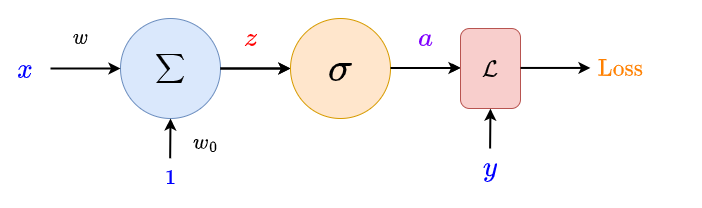
\includegraphics[width=90mm,scale=0.4]{images/nn_2_images/llc_as_neuron_loss.png}
        \end{figure}
        
        We want to link $\loss$ to $w$. In order to do that, we need to \textbf{connect} each thing in between.

        \begin{itemize}
            \item This lets us \textbf{combine} lots of simple \textbf{links} to get our more complicated result.
            \note{We can also call this "chaining together" lots of derivatives.}
        \end{itemize}

        \phantom{}
        
        Loss \org{$\loss$} is what we really care about. So, what is the loss directly \textbf{connected} to? The \textbf{activation}, \purp{$a$}.

        \begin{itemize}
            \item Our loss function $\loss(a,y)$ contains information about how $\loss$ is linked to $a$.
        \end{itemize}
        
        
        
        \begin{equation}
            \overbrace{
                \pderiv {\org{\loss}} {\pur{a}} 
            }^{\text{Loss unit}} 
        \end{equation}

        We send this information backwards, so it can be used later.

        \begin{figure}[H]
            \centering
            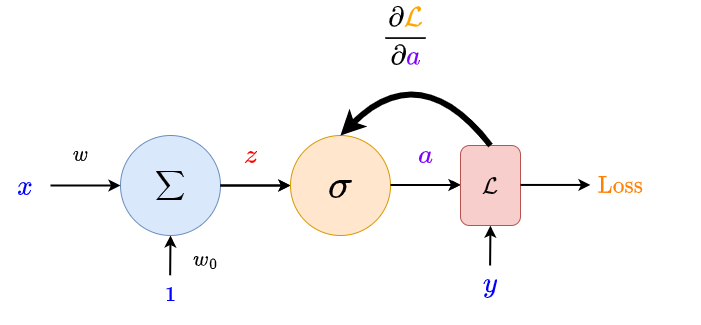
\includegraphics[width=90mm,scale=0.4]{images/nn_2_images/llc_backprop_1.png}
        \end{figure}

        Now, we're on the $\sigma(z)$ unit.

        \begin{itemize}
            \item The $\sigma(z)$ unit contains information about how \pur{$a$} is linked to \red{$z$}.

            \item We've connected \org{$\loss$} to \pur{$a$}, and \pur{$a$} to \red{$z$}. We chain them together, connecting \org{$\loss$} to \red{$z$}.

                \begin{equation}
                    \overbrace{
                        \pderiv {\org{\loss}} {\pur{a}} 
                    }^{\text{Loss unit}}
                    \cmul
                    \overbrace{
                        \pderiv {\pur{a}}     {\red{z}}
                    }^{\text{Activation function}}
                \end{equation}
        \end{itemize}
        
        We haven't reached $w$ yet, so we send this information further back.
        
        \begin{figure}[H]
            \centering
            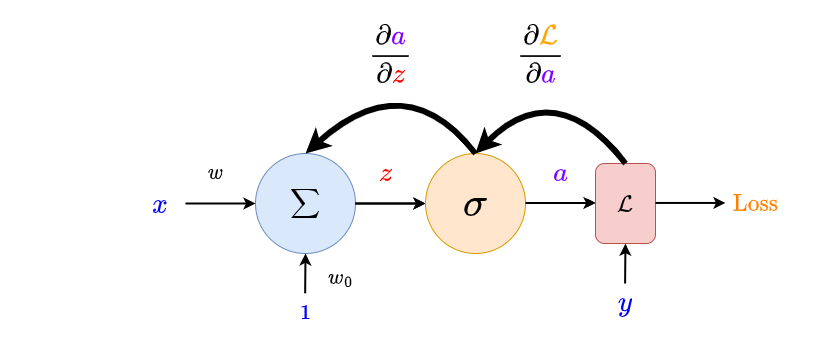
\includegraphics[width=100mm,scale=0.4]{images/nn_2_images/llc_backprop_2.png}
        \end{figure}

        
        
        Finally, we reach $\sum$.

        \begin{itemize}
            \item The $\sum$ unit contains information about how $z$ is linked to $w$.
            \item Finally, we have a chain of links, that allows us to connect \org{$\loss$} to $w$.
        \end{itemize}

        This last derivative uses $x$, because $w^Tx +w_0 = z$.

        \begin{figure}[H]
            \centering
            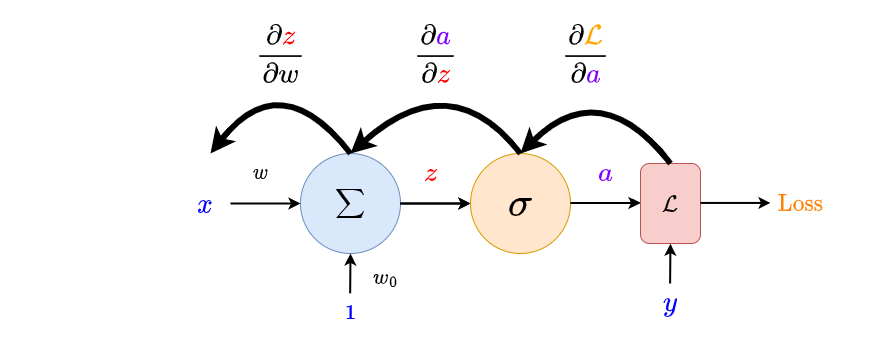
\includegraphics[width=110mm,scale=0.4]{images/nn_2_images/llc_backprop_3.png}
        \end{figure}
        
        And, we built our chain rule! This contains the \textbf{information} of the derivatives from \textbf{every} unit.
        
        \begin{equation}
            \pderiv {\pur{\loss}} {w} 
            =
            \overbrace{
                \pderiv {\pur{\loss}} {\blu{a}} 
            }^{\text{Loss unit}}
            \cmul
            \overbrace{
                \pderiv {\blu{a}}     {\red{z}}
            }^{\text{Activation}}
                \cmul
            \overbrace{
                \pderiv {\red{z}}     {w}
            }^{\text{Linear subunit}}
        \end{equation}
        
        Moving backwards like this is called \textbf{back-propagation}.\\
        
        \begin{definition}
            \vocab{Back-propagation} is the process of moving "\gren{backwards}" through your network, starting at the \purp{loss} and moving back layer-by-layer, and gathering terms in your \purp{chain rule}.
            
            We call it "\purp{propagation}" because we send backwards the \gren{terms} of our chain rule about later derivatives.
            
            An \gren{earlier} unit (closer to the "left") has all of the \purp{derivatives} that come after (to the "right" of) it, along with its own term.
        \end{definition}
        
    \phantom{}
    
    \subsection{Summary of neural network gradient descent: a high-level view}
    
        So, with just this, we have built up the basic idea of how we \textbf{train} our model: now that we have the gradient, we can do \textbf{gradient descent} like we normally do!
            \note{This summary covers some things we haven't fully discussed. We'll continue digging into the topic!}\\
        
        \begin{concept}
            We can do \vocab{gradient descent} on a \vocab{neural network} using the ideas we've built up:
            
            \begin{itemize}
                \item Do a \vocab{forward pass}, where we compute the value of each \gren{unit} in our model, passing the information \purp{forward} - each layer's \textbf{output} is the next layer's \textbf{input}.
                    \begin{itemize}
                        \item We finish by getting the \purp{loss}.
                    \end{itemize}
                    
            \phantom{}
                    
                \item Do \vocab{back-propagation}: build up a \purp{chain rule}, starting at the \purp{loss} function, and get each unit's \gren{derivative} in \purp{reverse order}.
                    \begin{itemize}
                        \item \purp{Reverse} order: if you have 3 layers, you want to get the 3rd layer's \gren{derivatives}, then the 2nd layer, then the 1st.
                        
                        \item \purp{Each weight} vector has its own \gren{gradient}: we'll deal with this later, but we need to calculate one for each of them.
                    \end{itemize}
                    
            \phantom{}
                
                \item Use your chain rule to get the \purp{gradient} $\pderiv{\loss}{w}$ for your \gren{weight} vector(s). Take a \vocab{gradient descent} step.
                
                \item \vocab{Repeat} until satisfied, or your model \purp{converges}.
            \end{itemize}
        \end{concept}
        
    \phantom{}
    
    \subsection{A two-neuron network: starting backprop}
        
        Above, we mention "\textbf{each} layer": we'll now transition to a \textbf{two-neuron} system, so we have "two layers". Then, we'll build up to many layers.
        
        Remember, though, that the \textbf{ideas} represented here are just extensions of what we did \textbf{above}.
        
        Let's get a look at our \textbf{two-neuron} system, now with our \textbf{loss} unit:
        
        \begin{figure}[H]
            \centering
            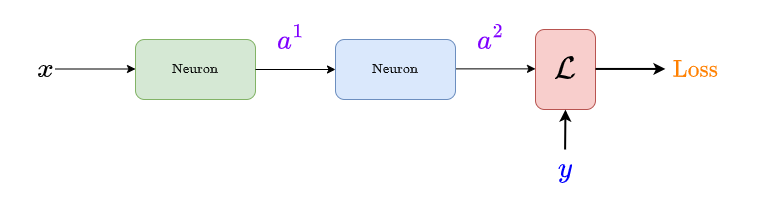
\includegraphics[width=140mm,scale=0.4]{images/nn_2_images/two_neurons_bp.png}
        \end{figure}
        
        And unpack it:
        
        \begin{figure}[H]
            \centering
            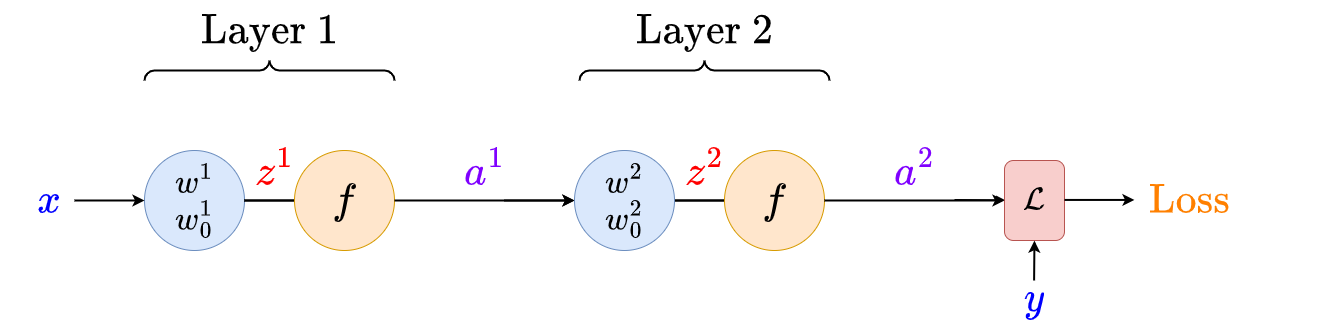
\includegraphics[width=140mm,scale=0.4]{images/nn_2_images/two_neurons_inside_bp.png}
        \end{figure}
        
        We want to do \textbf{back-propagation} like we did before. This time, we have \textbf{two} different layers of weights: $w^1$ and $w^2$. Does this cause any problems?
        
        It turns out, it doesn't! We mentioned in the first part of chapter 7 that we can treat the \textbf{output} of the \textbf{first} layer $a^1$ as the same as if it were an \textbf{input} $x$.
            \note{This is one of the biggest benefits of neural network layers!}
            
        \begin{figure}[H]
            \centering
            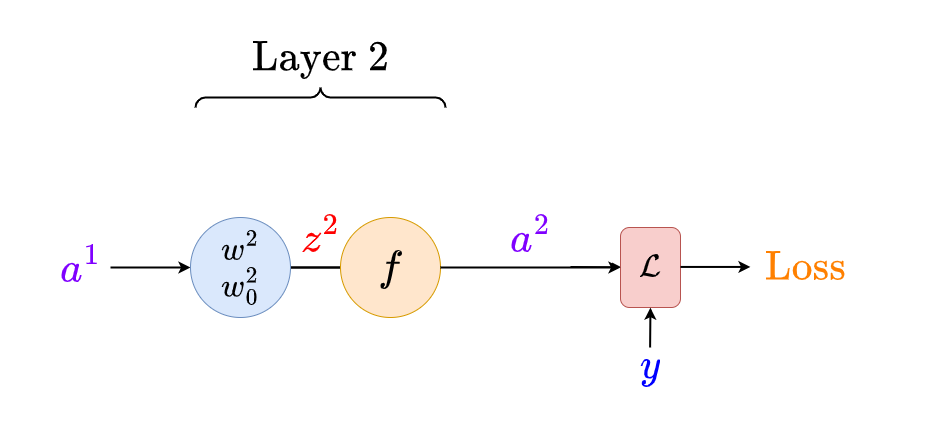
\includegraphics[width=90mm,scale=0.4]{images/nn_2_images/layer2_bp.png}
        \end{figure}
        
        Now, we can do backprop safely.
            \note{"Backprop" is a common shortening of "back-propagation".}
        
        \begin{figure}[H]
            \centering
            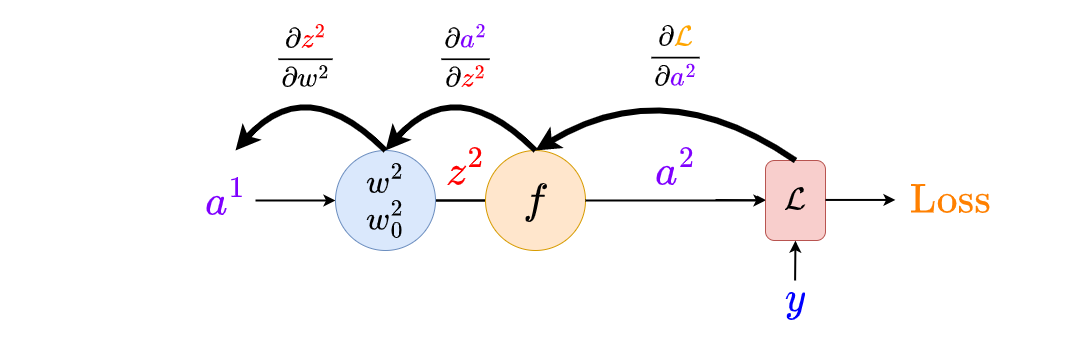
\includegraphics[width=120mm,scale=0.4]{images/nn_2_images/layer2_bp1.png}
        \end{figure}
        
        We can get:
        
        \begin{equation}
            \pderiv {\org{\loss}} {w^2} 
            =
            \overbrace{
                \pderiv {\org{\loss}} {\pur{a^2}} 
            }^{\text{Loss unit}}
            \cmul
            \overbrace{
                \pderiv {\pur{a^2}}     {\red{z^2}}
            }^{\text{Activation}}
                \cmul
            \overbrace{
                \pderiv {\red{z^2}}     {w^2}
            }^{\text{Linear}}
        \end{equation}
        
        The same format as for our \textbf{one-neuron} system! We now have a gradient we can update for our \textbf{second} weight vector.
        
        But what about our \textbf{first} weight vector?
        
    \phantom{}
    
    \subsection{Continuing backprop: One more problem}
    
        We need to continue further to reach our \textbf{earlier} weights: this is why we have to work \textbf{backward}.\\
        
        \begin{concept}
            We work \purp{backward} in \vocab{back-propagation} because every layer after the \gren{current} one \purp{affects} the gradient.
            
            Our current layer \gren{feeds} into the next layer, which feeds into the layer after that, and so on. So this layer affects \purp{every} later layer, which then affect the loss.
            
            So, to see the effect on the \purp{output}, we have to \gren{start} from the \purp{loss}, and get every layer \purp{between} it and our weight vector.
        \end{concept}
            
            \note{Remember that when we say "$f$ feeds into $g$", we mean that the output of $f$ is the input to $g$.}
            
        \phantom{ }
            
        \begin{figure}[H]
            \centering
            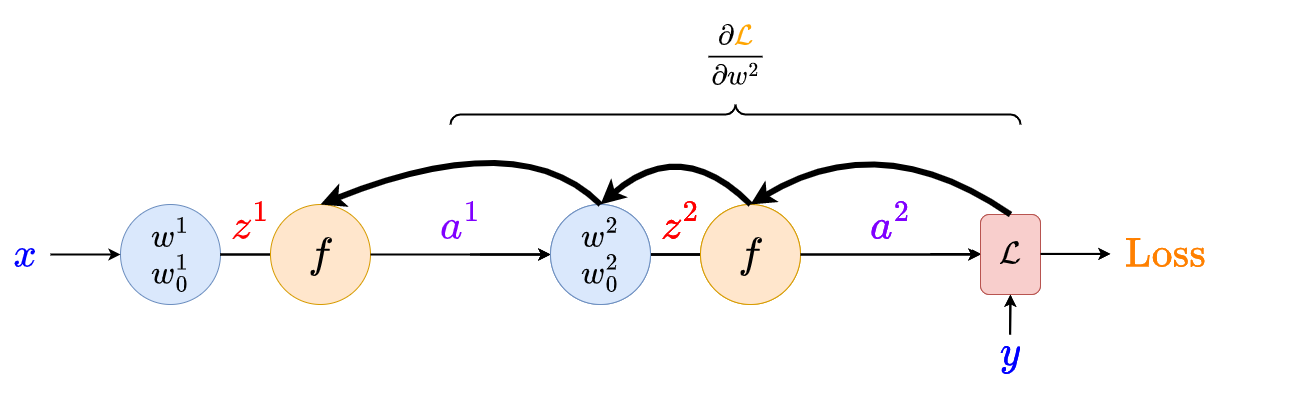
\includegraphics[width=120mm,scale=0.4]{images/nn_2_images/two_neurons_inside_bp2.png}
        \end{figure}
            
        We have one problem, though: 
        
        We just gathered the derivative $\pderivslash {\pur{\loss}} {w^2} $. If we wanted to continue the chain rule, we would expect to add more terms, like:
            \note{Since our current derivative includes $w^2$, we would continue it with a $w^2$ in the 
            "top" of a derivative, 
            $$\pderiv{\pur{\loss}}{w^2} \pderiv{w^2}{r}$$
            We're not sure what "$r$" is yet.}
        
        \begin{equation}
            \pderiv{w^2}{a^1}
        \end{equation}
        
        The problem is, what is $w^2$? It's a vector of constants.
        
        \begin{equation}
            w^2 = 
            \begin{bmatrix}
                    w_1^2 \\ w_2^2 \\ \vdots \\ w_n^2
            \end{bmatrix}
            ,
            \qquad
            \qquad
            \text{Not a function of $a^1$!}
        \end{equation}
        
        That derivative above is going to be \textbf{zero}! In other words, $w^2$ isn't really the \textbf{input} to $z^2$: it's a \textbf{parameter}.
            \note{We were building our chain rule by combining inputs with outputs: that's what links two layers together.\\
            \phantom{ }\\
            So, it should make sense that using something like $w$ (that doesn't link two layers) prevents us from making a longer chain rule.}
            
        So, we can't end our derivative with $w^2$. Instead, we have to use something else. $z^2$'s real input is $a^1$, so let's go directly to that!
        
        \begin{figure}[H]
            \centering
            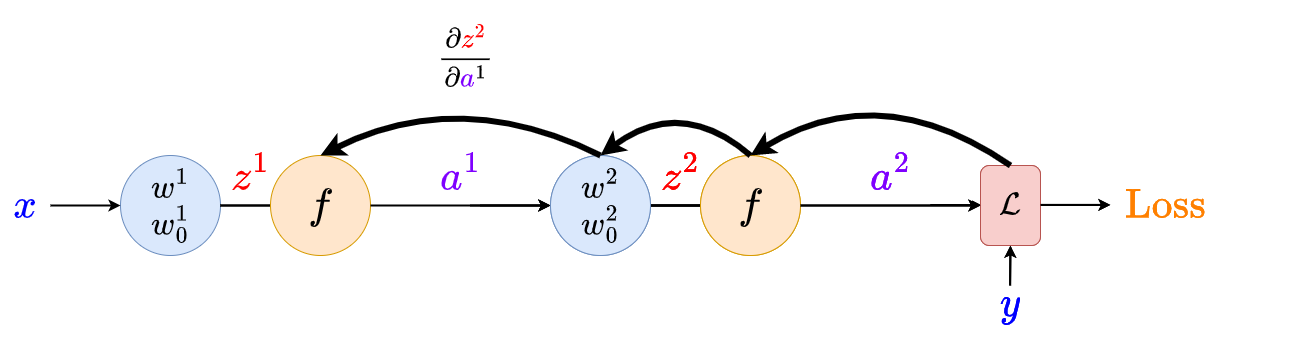
\includegraphics[width=120mm,scale=0.4]{images/nn_2_images/two_neurons_inside_bp3.png}
            \caption*{Using this allows us to move from layer 2 to layer 1.}
        \end{figure}
        
        Now, we have our new chain rule:
        
        \begin{equation}
            \pderiv {\org{\loss}} {a^1} 
            =
            \overbrace{
                \pderiv {\org{\loss}} {\pur{a^2}} 
                    \cmul
                \pderiv {\pur{a^2}}   {\red{z^2}}
            }^{\text{Other terms} } 
                \cmul
            \overbrace{
                \pderiv {\red{z^2}}   {a^1}
            }^{\text{Link Layers}}
        \end{equation}
        
        \begin{concept}
            For our \vocab{weight gradient} in layer $l$, we have to end our \purp{chain rule} with
            
            \begin{equation*}
                \pderiv {\red{z^\ell}}   {w^\ell}
            \end{equation*}
            
            So we can get 
            
            \begin{equation*}
                \pderiv {\org{\loss}} {w^\ell} 
                =
                \overbrace{
                    \pderiv {\org{\loss}} {\red{z^\ell}} 
                }^{\text{Other terms} }
                \cmul  
                \overbrace{
                    \pderiv {\red{z^\ell}}   {w^\ell}
                }^{\text{Get weight grad}}
            \end{equation*}
            
            However, because $w^l$ is not the \textbf{input} of layer $l$, we can't use it to find the gradient of \gren{earlier layers}.
            
            Instead, we use 
            
            \begin{equation}
                \pderiv {\red{z^\ell}}   {a^{\ell-1}}
            \end{equation}
            
            To "\purp{link together}" two different layers $\ell$ and $\ell-1$ in a \gren{chain rule}.
        \end{concept}
        
            \note{In this section, we compressed lots of derivatives into 
            $$\pderiv {\pur{\loss}} {\red{z^\ell}}$$
            Don't let this alarm you, this just hides our long chain of derivatives!}
            
    \phantom{}
    
    \subsection{Finishing two-neuron backprop}
    
        Now that we have safely connected our layers, we can do the rest of our gradient. First, let's lump together everything we did before:
        
        \begin{figure}[H]
            \centering
            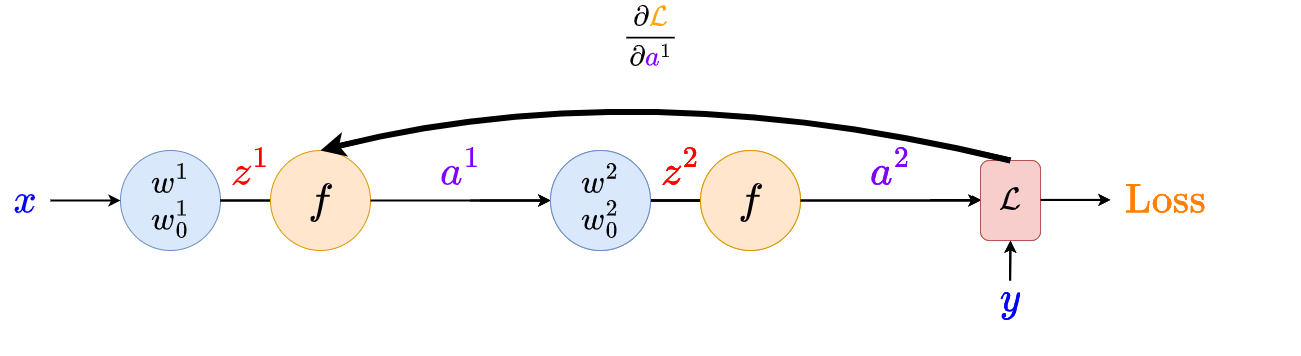
\includegraphics[width=120mm,scale=0.4]{images/nn_2_images/two_neurons_inside_bp4.png}
            \caption*{All the info we need is stored in this derivative: it can be written out using our friendly chain rule from earlier.}
        \end{figure}
        
        Now, we can add our remaining terms. It's the same as before: we want to look at the pre-activation
        
        \begin{figure}[H]
            \centering
            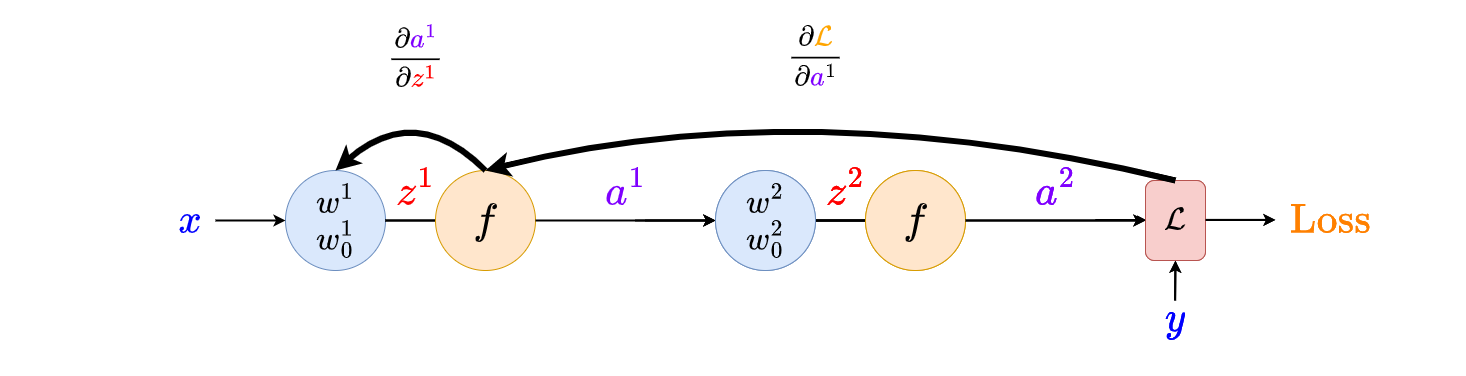
\includegraphics[width=120mm,scale=0.4]{images/nn_2_images/two_neurons_inside_bp5.png}
        \end{figure}
        
        And finally, our input:
        
        \begin{figure}[H]
            \centering
            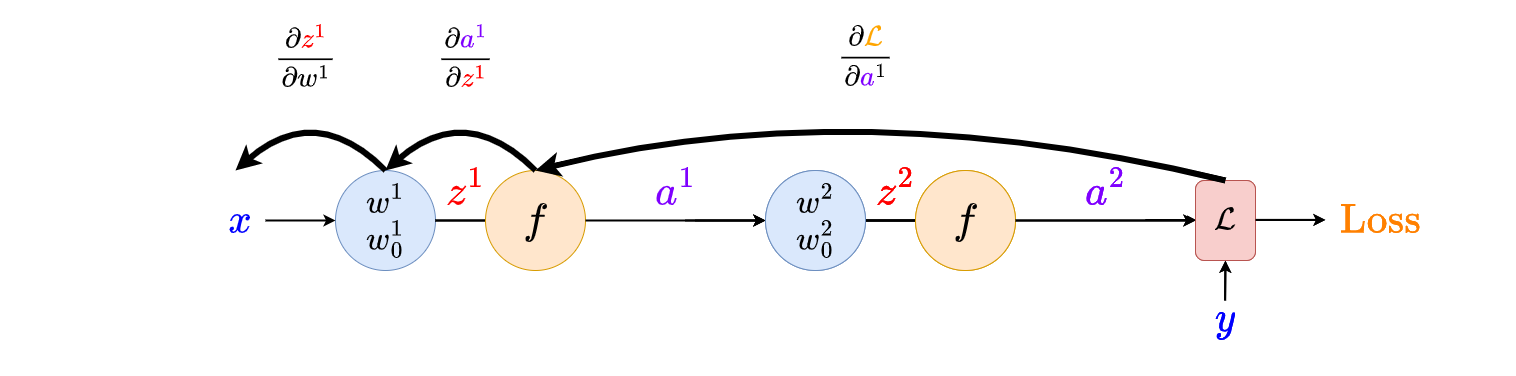
\includegraphics[width=120mm,scale=0.4]{images/nn_2_images/two_neurons_inside_bp6.png}
        \end{figure}
        
        We can get our second chain rule
        
        \begin{equation}
            \pderiv {\org{\loss}} {w^1} 
            =
            \overbrace{
                \pderiv {\org{\loss}} {\pur{a^1}} 
            }^{\text{Other layers}}
            \cmul
            \overbrace{
                \pderiv {\pur{a^1}}   {\red{z^1}}
                \cmul
                \pderiv {\red{z^1}}   {w^1}
            }^{\text{Layer 1}}
        \end{equation}
        
        Which, in reality, looks much bigger:
        
        \begin{equation}
            \pderiv {\org{\loss}} {w^1} 
            =
            \overbrace{
                \Bigg(
                    \pderiv {\org{\loss}} {\pur{a^2}} 
                \Bigg)
            }^{\text{Loss unit}}
            \cmul
            \overbrace{
                \Bigg(
                    \pderiv {\pur{a^2}}   {\red{z^2}}
                        \cmul
                    \pderiv {\red{z^2}}   {\blu{a^1}}
                \Bigg) 
            }^{\text{Layer 2}}
            \cmul
            \overbrace{
                \Bigg(
                    \pderiv {\blu{a^1}}   {\grn{z^1}}
                        \cmul
                    \pderiv {\grn{z^1}}   {w^1}
                \Bigg)
            }^{\text{Layer 1}}
        \end{equation}
        
        We see a clear \textbf{pattern} here! In fact, this is the procedure we'll use for a neural network with \textbf{any} number of layers.\\
        
        \begin{concept}
            We can get all of our \vocab{weight gradients} by repeatedly appending to the \purp{chain rule}.
            
            If we want to get the \orgg{weight gradient} of layer $\ell$, we \gren{terminate} with
            
            \begin{equation*}
                \overbrace{
                    \pderiv {\blu{a^\ell}} {\red{z^\ell}}
                }^{\text{Within layer}}
                    \cmul
                \overbrace{
                    \pderiv {\red{z^\ell}} {w^\ell}
                }^{\text{Get weight grad}}
            \end{equation*}
            
            If we want to \gren{extend} to the previous layer, we \redd{instead} multiply by
            
            \begin{equation*}
                \overbrace{
                    \pderiv {\blu{a^\ell}} {\red{z^\ell}}
                }^{\text{Within layer}}
                    \cmul
                \overbrace{
                    \pderiv {\red{z^\ell}} {a^{\ell-1}}
                }^{\text{Link layers}}
            \end{equation*}
            
        \end{concept}
        
    \phantom{}
    
    \subsection{Many layers: Doing back-propagation}
    
        Now, we'll consider the case of many possible layers.
            \note{To make it more readable, we'll use boxes instead of circles for units.}
            
        \phantom{ }
            
        \begin{figure}[H]
            \centering
            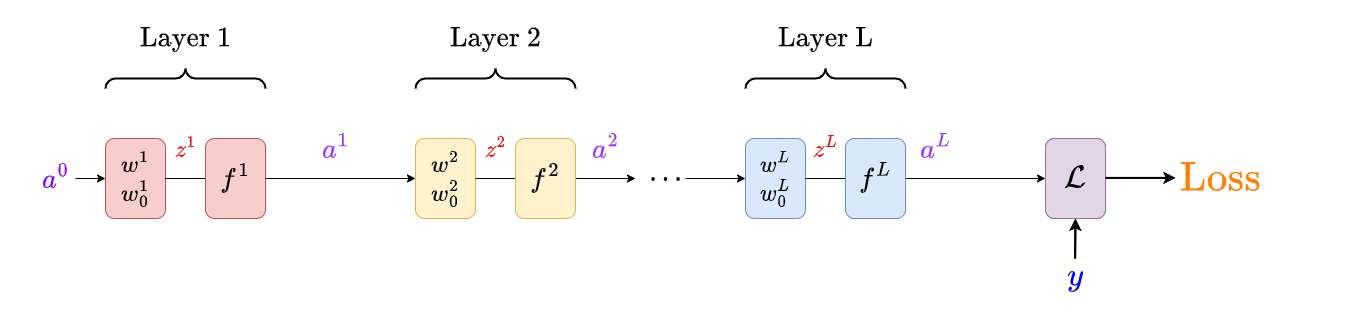
\includegraphics[width=180mm,scale=0.4]{images/nn_2_images/network_bp.png}
        \end{figure}
        
        This may look intimidating, but we already have all the tools we need to handle this problem.
        
        Our goal is to get a \textbf{gradient} for each of our \textbf{weight} vectors $w^\ell$, so we can do gradient descent and \textbf{improve} our model.
        
        According to our above analysis in Concept 9, we need only a few steps to get all of our gradients.
        
        \begin{concept}
            In order to do \vocab{back-propagation}, we have to build up our \vocab{chain rule} for each weight gradient.
            
            \begin{itemize}
                \item We start our chain rule with one term shared by every gradient: 
                    \begin{equation*}
                        \overbrace{
                            \pderiv {\pur{\loss}} {\blu{a^L}} 
                        }^{\text{Loss unit}}
                    \end{equation*}
            \end{itemize}
            
            Then, we follow these two steps until we run out of layers:
            \begin{itemize}
                \item We're at layer $\ell$. We want to get the \purp{weight gradient} for this layer. We get this by \gren{multiplying} our chain rule by
                
                    \begin{equation*}
                        \overbrace{
                            \pderiv {\blu{a^\ell}} {\red{z^\ell}}
                        }^{\text{Within layer}}
                            \cmul
                        \overbrace{
                            \pderiv {\red{z^\ell}} {w^\ell}
                        }^{\text{Get weight grad}}
                    \end{equation*}
                    
                    We \redd{exclude} this term for any other gradients we want.
                
                \item If we aren't at layer 1, there's a previous layer we want to get the weight for. We reach layer $\ell-1$ by multiplying our chain rule by 
                
                    \begin{equation*}
                        \overbrace{
                            \pderiv {\blu{a^\ell}} {\red{z^\ell}}
                        }^{\text{Within layer}}
                            \cmul
                        \overbrace{
                            \pderiv {\red{z^\ell}} {a^{\ell-1}}
                        }^{\text{Link layers}}
                    \end{equation*}
            \end{itemize}
            
            Once we reach layer 1, we have \gren{every single} weight vector we need! Repeat the process for $w_0$ gradients and then do \purp{gradient descent}.
        \end{concept}
        
        Let's get an idea of what this looks like in general:
        
        \begin{equation}
            \pderiv {\pur{\loss}} {w^\ell} 
            =
            \overbrace{
                \Bigg(
                    \pderiv {\pur{\loss}} {\blu{a^L}} 
                \Bigg)
            }^{\text{Loss unit}}
            \cmul
            \overbrace{
                \Bigg(
                    \pderiv {\blu{a^L}}   {\red{z^L}}
                        \cmul
                    \pderiv {\red{z^L}}   {\grn{a^{L-1}}}
                \Bigg) 
            }^{\text{Layer $L$}}
            \cmul
            \overbrace{
                \Bigg(
                    \pderiv {\blu{a^{L-1}}}   {\red{z^{L-1}}}
                        \cmul
                    \pderiv {\red{z^{L-1}}}   {\grn{a^{L-2}}}
                \Bigg) 
            }^{\text{Layer $L-1$}}
            \cmul
            \Bigg(
                \cdots 
            \Bigg)
            \cmul
            \overbrace{
                \Bigg(
                    \pderiv {\blu{a^\ell}}   {\red{z^\ell}}
                        \cmul
                    \pderiv {\red{z^\ell}}   {\org{w^{\ell}}}
                \Bigg) 
            }^{\text{Layer $\ell$}}
        \end{equation}
        
        That's pretty ugly. If we need to hide the complexity, we can:\\
        
        \begin{notation}
            If you need to do so for \purp{ease}, you can \orgg{compress}  your derivatives. For example, if we want to only have the last weight term \gren{separate}, we can do:
            
            \begin{equation*}
                \pderiv {\pur{\loss}} {w^\ell} 
                =
                \overbrace{
                    \pderiv {\pur{\loss}} {\red{z^\ell}} 
                }^{\text{Other}}
                \cmul
                \overbrace{
                    \pderiv {\red{z^\ell}}   {w^\ell}
                }^{\text{Weight term}}
            \end{equation*}
        \end{notation}
        
        But we should also explore what each of these terms \textit{are}.
        
    \phantom{}
    
    \subsection{What do these derivatives equal?}
    
        Let's look at each of these derivatives and see if we can't simplify them a bit.
        
        First, every gradient needs
        
        \begin{itemize}
            \item The \vocab{loss derivative}:
            
                \begin{equation}
                    \pderiv {\pur{\loss}} {\blu{a^L}}
                \end{equation}
                
                This \textbf{depends} on on our loss function, so we're \textbf{stuck} with that one.
            
        \end{itemize}
            
        Next, within each layer, we have
        
        \begin{itemize}
            \item The \vocab{activation function} - between our activation $a$ and preactivation $z$:
            
                \begin{equation}
                    \pderiv {\blu{a^\ell}}   {\red{z^\ell}}
                \end{equation}
                
                What does the function between these \textbf{look} like?
                
                \begin{equation}
                    \blu{a} = f(\red{z})
                \end{equation}
                
                Well, that's not super interesting: we \textbf{don't know }our function. But, at least we can \textbf{write} it using $f$: that way, we know that this term only depends on our \textbf{activation} function.
                
                \begin{equation}
                    \pderiv {\blu{a^\ell}}   {\red{z^\ell}} 
                    = 
                    \overbrace{
                    \Big(
                        f^\ell 
                    \Big)'
                    }^{\text{deriv of func for layer $\ell$}}
                    \overbrace{
                    (
                        \red{z^\ell}
                    )
                    }^{\text{Deriv input}}
                \end{equation}
                
                This expression is a bit visually clunky, but it works. Without the annotation:
                    \note{$z^\ell$ is not being multiplied by $(f^\ell)'$, it's the input to that derivative.}

                \begin{equation}
                    \pderiv {\blu{a^\ell}}   {\red{z^\ell}} 
                    = 
                    \Big(
                        f^\ell 
                    \Big)'
                    (
                        \red{z^\ell}
                    )
                \end{equation}
                
        \end{itemize}
        
    Between layers, we have
        
        \begin{itemize}
            
            \item We can also think about the derivative of the \vocab{linear function} that \textbf{connects two layers}:
                \note{Be careful not to get this mixed up with the last one!\\
                They look similar, but one is within the layer, and the other is between layers.}
            
                \begin{equation}
                    \pderiv {\red{z^\ell}}   {\blu{a^{\ell-1}}}
                \end{equation}
                
                So, we want the function of these two:
                
                \begin{equation}
                    \red{z^\ell} = w^\ell \blu{ a^{\ell-1} } + w_0^\ell
                \end{equation}
                
                This one is pretty simple! We just take the derivative manually:
                
                \begin{equation}
                    \pderiv {\red{z^\ell}}   {\blu{a^{\ell-1}}}
                    =
                    w^{\ell}
                \end{equation}
                
        \end{itemize}
        
    Finally, every gradient will end with...
        
        \begin{itemize}
                
            \item The derivative that directly connects to a \textbf{weight}, again using the \vocab{linear function}:
            
                \begin{equation}
                    \pderiv {\red{z^\ell}}   {w^{\ell}}
                \end{equation}
                
                The linear function is the same:
            
                \begin{equation}
                    \red{z^\ell} = w^\ell \blu{ a^{\ell-1} } + w_0^\ell
                \end{equation}
                
                But with a different \textbf{variable}, the \textbf{derivative} comes out different:
                
                \begin{equation}
                    \pderiv {\red{z^\ell}}   {w^{\ell}}
                    =
                    a^{\ell-1} 
                \end{equation}
                
        \end{itemize}
        
    \begin{notation}
        Our \vocab{derivatives} for the \purp{chain rule} in a \vocab{1-D neural network} take the form:
        
        \begin{equation*}
            \pderiv {\pur{\loss}} {\blu{a^L}}
        \end{equation*}
        
        \begin{equation*}
            \pderiv {\blu{a^\ell}}   {\red{z^\ell}} = (f^\ell)'(\red{z^\ell})
        \end{equation*}
        
        \begin{equation*}
            \pderiv {\red{z^\ell}}   {\blu{a^{\ell-1}}}
            =
            w^{\ell}
        \end{equation*}
        
        \begin{equation*}
            \pderiv {\red{z^\ell}}   {w^{\ell}}
            =
            a^{\ell-1} 
        \end{equation*}
    \end{notation}

    Now, we can rewrite our generalized expression for gradient:
    
    
        \begin{equation}
            \pderiv {\pur{\loss}} {w^\ell} 
            =
            \overbrace{
                \Bigg(
                    \pderiv {\pur{\loss}} {\blu{a^L}} 
                \Bigg)
            }^{\text{Loss unit}}
            \cmul
            \overbrace{
                \Bigg(
                    (f^L)'(\red{z^L})
                        \cmul
                    w^L
                \Bigg) 
            }^{\text{Layer $L$}}
            \cmul
            \overbrace{
                \Bigg(
                    (f^{L-1})'(\red{z^{L-1}})
                        \cmul
                    w^{L-1}
                \Bigg) 
            }^{\text{Layer $L-1$}}
            \cmul
            \Bigg(
                \cdots 
            \Bigg)
            \cmul
            \overbrace{
                \Bigg(
                    (f^\ell)'(\red{z^\ell})
                        \cmul
                    a^{\ell-1}
                \Bigg) 
            }^{\text{Layer $\ell$}}
        \end{equation}
        
        Our expressions are more concrete now. It's still pretty visually messy, though.
        
    \phantom{}
    
    \subsection{Activation Derivatives}
    
        We weren't able to \textbf{simplify} our expressions above, partly because we didn't know which \textbf{loss} or \textbf{activation} function we were going to use.
        
        So, here, we will look at the \textbf{common} choices for these functions, and \textbf{catalog} what their derivatives look like.
        
        \begin{itemize}
            \item \vocab{Step function} step$(z)$:
            
                \begin{equation}
                    \deriv{}{z} \text{step}(z) = 0
                \end{equation}
                
                This is part of why we don't use this function: it has no gradient. We can show this by looking piecewise:
                
                \begin{equation}
                    \text{step}(z) 
                    =
                    \begin{cases}
                      \blu{1} & \text{if $z \geq 0$}\\
                      \blu{0} & \text{if $z < 0$}
                    \end{cases}
                \end{equation}
                
                And take the derivative of each piece:
                
                \begin{equation}
                    \deriv{}{z} \text{ReLU}(z)
                    =
                    0
                    =
                    \begin{cases}
                      \red{0} & \text{if $z \geq 0$}\\
                      \red{0} & \text{if $z < 0$}
                    \end{cases}
                \end{equation}
        
            \item \vocab{Rectified Linear Unit} ReLU$(z)$:
            
                \begin{equation}
                    \deriv{}{z} \text{ReLU}(z) = \text{step}(z)
                \end{equation}
                
                This one might be a bit surprising at first, but it makes sense if you \textbf{also} break it up into cases:
                
                \begin{equation}
                    \text{ReLU}(z) 
                    =
                    \max(0,z)
                    =
                    \begin{cases}
                      \blu{z} & \text{if $z \geq 0$}\\
                      \blu{0} & \text{if $z < 0$}
                    \end{cases}
                \end{equation}
                
                And take the derivative of each piece:
                
                \begin{equation}
                    \deriv{}{z} \text{ReLU}(z)
                    =
                    \text{step}(z) 
                    =
                    \begin{cases}
                      \red{1} & \text{if $z \geq 0$}\\
                      \red{0} & \text{if $z < 0$}
                    \end{cases}
                \end{equation}
               
                
            \item \vocab{Sigmoid} function $\sigma(z)$:
            
                \begin{equation}
                    \deriv{}{z}\sigma(z) 
                    =
                    \sigma(z)(1-\sigma(z))
                    =
                    \frac{e^{-z}}{(1+e^{-z})^2}
                \end{equation}
                
                This derivative is useful for simplifying NLL, and has a nice form.
                    \note{We can just compute the derivative with the single-variable chain rule.}
                    
                As a reminder, the function looks like:
                
                \begin{equation}
                    \sigma(z) 
                    =
                    \frac{1}{1+e^{-z}}
                \end{equation}
                
            \item \vocab{Identity} ("linear") function $f(z)=z$:
            
                \begin{equation}
                    \deriv{}{z} z
                    =
                    1
                \end{equation}
                
                This one follows from the definition of the derivative.
                
                We cannot rely on a linear activation function for our \textbf{hidden} layers, because a linear neural network is no more \textbf{expressive} than one layer.
                
                But, we use it as the output activation for \textbf{regression}.
                
            \item \vocab{Softmax} function softmax$(z)$:
            
                This function has a difficult derivative we won't go over here. 
                    \note{If you're curious, here's a \href{https://towardsdatascience.com/derivative-of-the-softmax-function-and-the-categorical-cross-entropy-loss-ffceefc081d1}{link}. }
                
            \item \vocab{Hyperbolic tangent} function $\tanh(z)$:
            
                \begin{equation}
                    \deriv{}{z}\tanh(z)
                    =
                    1 - \tanh(z)^2
                \end{equation}
                
                This strange little expression is 1 minus the "hyperbolic secant" squared. We won't bother further with it.\\
        \end{itemize}
        
        
        \begin{notation}
            For our various \vocab{activation} functions, we have the \vocab{derivatives}:
            
            Step:
            
            \begin{equation*}
                \deriv{}{z} \text{step}(z) = 0
            \end{equation*}
            
            ReLU:
            
            \begin{equation*}
                \deriv{}{z} \text{ReLU}(z) = \text{step}(z)
            \end{equation*}
            
            Sigmoid:
            
            \begin{equation*}
                \deriv{}{z}\sigma(z) 
                =
                \sigma(z)(1-\sigma(z))
            \end{equation*}
            
            Identity/Linear:
            
            \begin{equation*}
                \deriv{}{z} z 
                =
                1
            \end{equation*}
        \end{notation}
        
    \phantom{}
    
    \subsection{Loss derivatives}
    
        Now, we look at the loss derivatives.
        
        \begin{itemize}
            \item \vocab{Square loss} function $\loss_{sq} = (a-y)^2$:
            
                \begin{equation}
                    \deriv{}{a} \loss_{sq} = 2(a-y)
                \end{equation}
                
                Follows from chain rule+power rule, used for regression.
                
            \item \vocab{Linear loss} function $\loss_{sq} = |a-y|$:
            
                \begin{equation}
                    \deriv{}{a} \loss_{lin} = \text{sign}(a-y)
                \end{equation}
                
                This one can also be handled piecewise, like step$(z)$ and ReLU$(z)$:
                
                \begin{equation}
                    |u| 
                    =
                    \begin{cases}
                      \blu{u} & \text{if $z \geq 0$}\\
                      \blu{-u} & \text{if $z < 0$}
                    \end{cases}
                \end{equation}
                
                We take the piecewise derivative:
                
                \begin{equation}
                    \deriv{}{u}
                    |u|
                    =
                    \text{sign}(u) 
                    =
                    \begin{cases}
                      \red{1} & \text{if $z \geq 0$}\\
                      \red{-1} & \text{if $z < 0$}
                    \end{cases}
                \end{equation}
                
            \item \vocab{NLL} (Negative-Log Likelihood) function $\loss_{NLL} = -( y \log(a) + (1-y) \log(1-a) )$
            
                \begin{equation}
                    \deriv{}{a} \loss_{NLL} = - \Bigg( \frac{y}{a} - \frac{1-y}{1-a} \Bigg)
                \end{equation}
            
            \item \vocab{NLLM} (Negative-Log Likelihood Multiclass) function $\loss_{NLL} = - \sum_j y_jlog(a_j)$
            
                Similar to softmax, we will omit this derivative.\\
        \end{itemize}
        
        \begin{notation}
            For our various \vocab{loss} functions, we have the \vocab{derivatives}:
            
            Square:
            
            \begin{equation*}
                \deriv{}{a} \loss_{sq} = 2(a-y)
            \end{equation*}
            
            Linear (Absolute):
            
            \begin{equation*}
                \deriv{}{a} \loss_{lin} = \text{sign}(a-y)
            \end{equation*}
            
            NLL (Negative-Log Likelihood):
            
            \begin{equation*}
                \deriv{}{a} \loss_{NLL} = - \Bigg( \frac{y}{a} - \frac{1-y}{1-a} \Bigg)
            \end{equation*}
        \end{notation}
        
    \phantom{}
    
    \subsection{Many neurons per layer}
    
        Now, we just have left the elephant in the room: what do we do about the case where we have \textit{big} layers? That is, what if we have \textbf{multiple} neurons per layer? This makes this more complex.
        
        Well, the solution is the same as earlier in the course: we introduce \textbf{matrices}.
        
        But this time, with a twist: we have to do serious \textbf{matrix} calculus: a difficult topic indeed.
        
        To handle this, we will go in somewhat \textbf{reversed} order, but one that better fits our needs.
        
        \begin{itemize}
            \item We begin by considering how the chain rule looks when we switch to matrix form.
            \item We give a general idea of what matrix derivatives look like.
            \item We list some of the results that matrix calculus gives us, for particular derivatives.
            \item We actually reason about how matrix calculus \textit{works}.
        \end{itemize}
        
        The last of these is by far the \textbf{hardest}, and warrants its own section. Nevertheless, even without it, you can more or less get the idea of what we need - hence why we're going in reversed order.

    \phantom{}
    
    \subsection{The chain rule: Matrix form}
    
        Let's start with the first: the punchline, how does the chain rule and our gradient descent \textbf{change} when we add \vocab{matrices}?
        
        It turns out, not much: by using \textbf{layers} in the last section, we were able to create a pretty powerful and mathematically \textbf{tidy} object.

        \begin{itemize}
            \item With layers, each layer feeds into the \textbf{next}, with no other interaction. And neurons \purp{within} the same layer do \gren{not} directly \gren{interact} with each other, which simplifies our math greatly.

            \begin{itemize}
                \item Basically, we have a bunch of functions (neurons) that, within a layer, have \gren{nothing} to do with each other, and only \textbf{output} to the \textbf{next} layer of similar functions. 
            \end{itemize}

            
            
            \item So, we can often \textbf{oversimplify} our model by thinking of each \purp{layer} as like a "big" function, taking in a vector of size \blu{$m^\ell$} and outputting a vector of size \red{$n^\ell$}. 
        \end{itemize}
        
        
        
        
        
        
        
        Our main concern is making sure we have agreement of \textbf{dimensions}!
            \note{In fact, if you just rearranging your matrices and transposing them can be a helpful way to debug. Be careful, though!}
    
        So, here's how our model looks now:
        
        \begin{figure}[H]
            \centering
            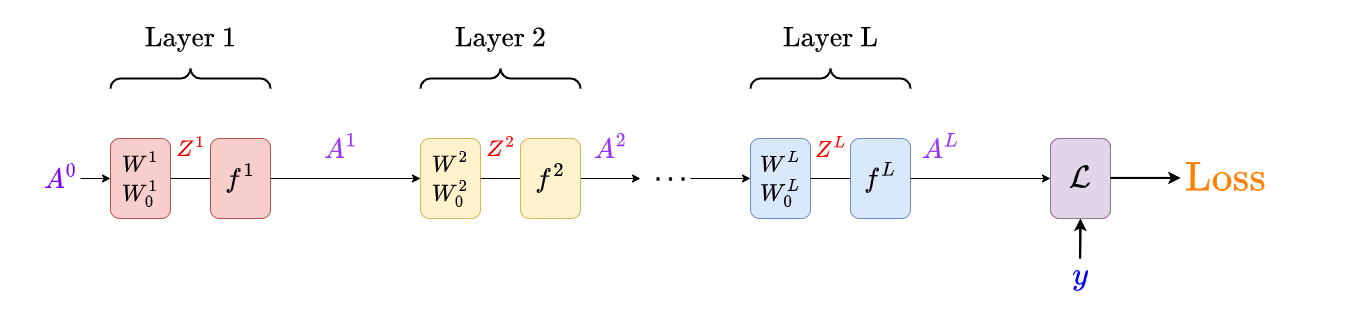
\includegraphics[width=180mm,scale=0.4]{images/nn_2_images/network_bp_full.png}
            \caption*{Pretty much the same! Only major difference: swapped scalars for vectors, and vectors for matrices (represented by switching to uppercase)}
        \end{figure}
        
        And, we do backprop the same way, too.
        
        Here, we're not going to explain much as we go: all we're doing is getting the \textbf{derivatives} we need for our \textbf{chain rule}! 
        
        As we go \textbf{backwards}, we can build the gradient for each \textbf{weight} we come across, in the way we described above.
        
        As always, we start from the loss function:
        
        \begin{figure}[H]
            \centering
            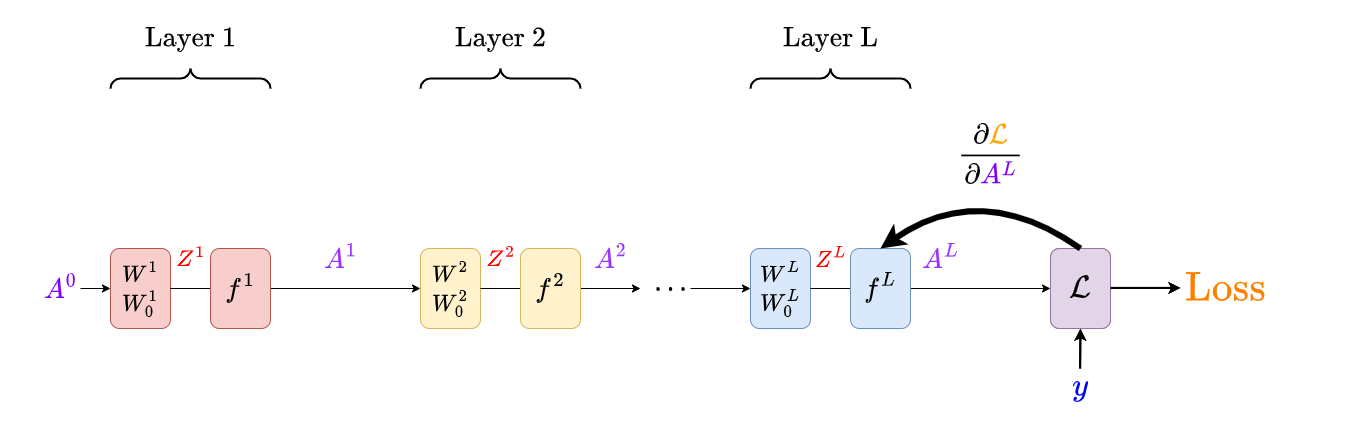
\includegraphics[width=180mm,scale=0.4]{images/nn_2_images/network_bp_full1.png}
        \end{figure}
        
        Take another step:
        
        \begin{figure}[H]
            \centering
            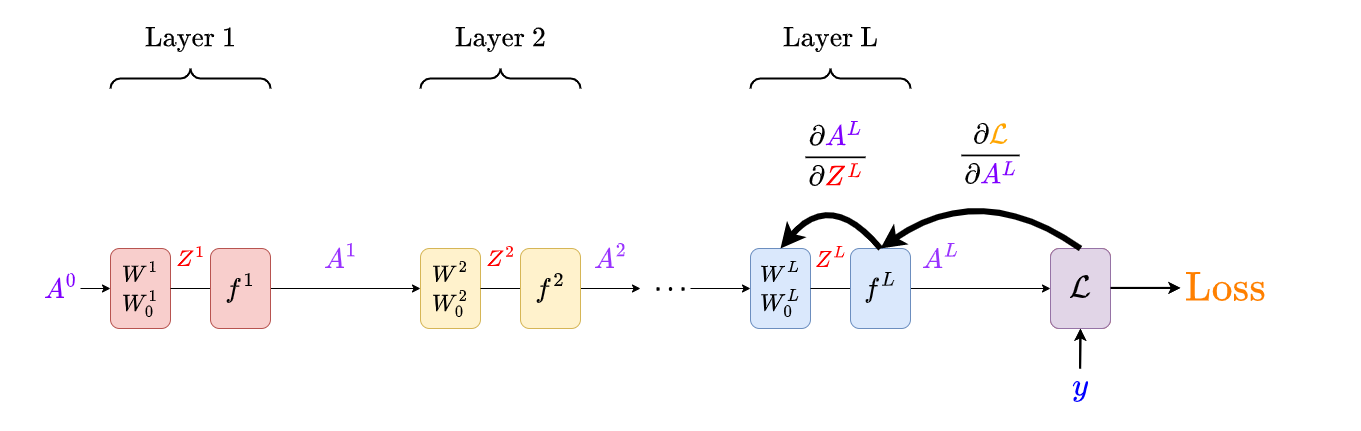
\includegraphics[width=180mm,scale=0.4]{images/nn_2_images/network_bp_full2.png}
        \end{figure}
        
        We'll pick up the pace: we'll jump to layer 2 and get its gradient.
            \note{The term $\pderivslash{\red{Z^L}}{\pur{A^2}}$ contains lots of derivatives from every layer between $L$ and 2. \\
            
            But, all we're omitting is the same kinds of steps we're doing in layers 1, 2, and L.}
        
        \begin{figure}[H]
            \centering
            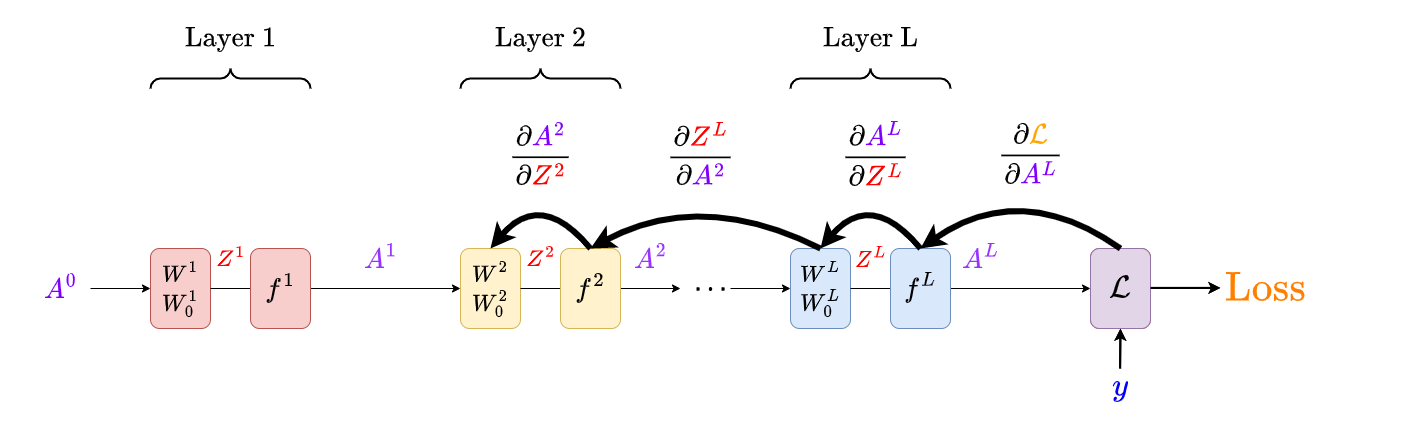
\includegraphics[width=180mm,scale=0.4]{images/nn_2_images/network_bp_full3.png}
        \end{figure}
        
        Now, we finally get to layer 1!
        
        \begin{figure}[H]
            \centering
            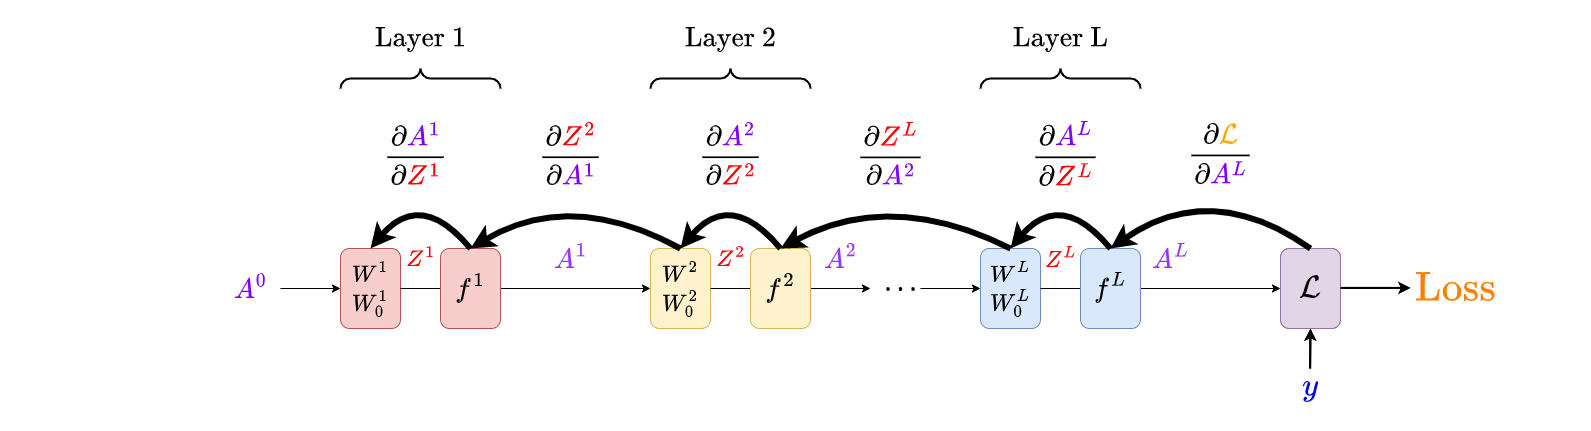
\includegraphics[width=180mm,scale=0.4]{images/nn_2_images/network_bp_full4.png}
        \end{figure}
        
        We finish off by getting what we're after: the gradient for $W^1$.\\
        
        \begin{notation}
            We depict neural network gradient descent using the below diagram (outside the box):
            
            The \gren{right}-facing \gren{straight} arrows come \purp{first}: they're part of the \vocab{forward pass}, where we get all of our values.
            
            The \gren{left}-facing \gren{curved} arrows come \purp{after}: they represent the \vocab{back-propagation} of the gradient.
        \end{notation}
        
        \begin{figure}[H]
            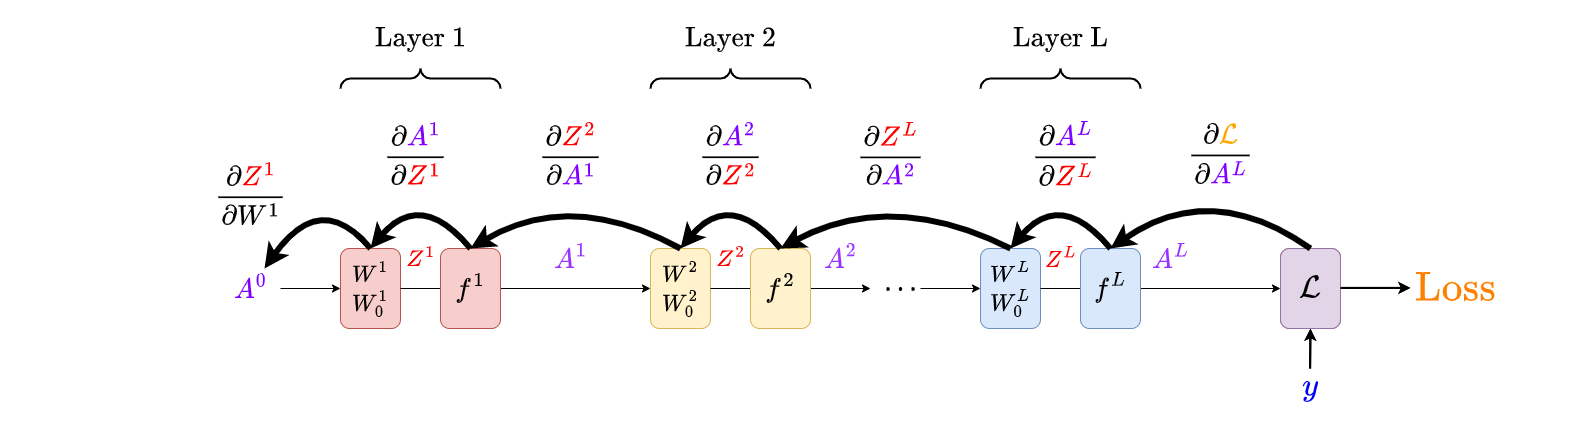
\includegraphics[width=180mm,scale=0.4]{images/nn_2_images/network_bp_full5.png}
        \end{figure}
        
        And, with this, we can rewrite our general equation for neural network gradients.
        
    \phantom{}
    
    \subsection{How the Chain Rule changes in Matrix form}
        
        As we discussed before, we can't just add onto our weight gradient to reach another layer: the final term
        
        \begin{equation}
            \pderiv{Z^\ell}{W^\ell}
        \end{equation}
        
        Ends our chain rule when we add it: $W^\ell$ isn't part of the input or output, so it doesn't connect to the previous layer.
        
        So, for this section, we'll add it \textbf{separately} at the end of our chain rule:
        
        \begin{equation*}
            \pderiv {\pur{\loss}} {W^\ell} 
            =
            \overbrace{
                \pderiv {\red{Z^\ell}}   {W^{\ell}}
            }^{\text{Weight link}} 
                \cmul
            \overbrace{
                \Bigg(
                    \pderiv {\pur{\loss}} {\red{Z^\ell}}
                \Bigg)^T
            }^{\text{Other layers}}
        \end{equation*}
        
        That way, we can add onto $\pderivslash {\pur{\loss}} {\red{Z^\ell}}$ without worrying about the weight derivative.
            
        Notice two minor changes caused by the switch to matrices:
        
        \begin{itemize}
            \item The order has to be \textbf{reversed}.
            \item We also have to do some weird \textbf{transposing}.
        \end{itemize}
        
        Both of these mostly boil down to trying to be careful about \textbf{shape}/dimension agreement.
            \note{There are also deeper interpretations, but they aren't worth digging into for now.}\\
        
        \begin{notation}
            The \vocab{gradient} $\nabla_{W^\ell} \loss$ for a neural network is given as:
            
            \begin{equation*}
                \pderiv {\pur{\loss}} {W^\ell} 
                =
                \overbrace{
                    \pderiv {\red{Z^\ell}}   {W^{\ell}}
                }^{\text{Weight link}} 
                    \cmul
                \overbrace{
                    \Bigg(
                        \pderiv {\pur{\loss}} {\red{Z^\ell}}
                    \Bigg)^T
                }^{\text{Other layers}}
            \end{equation*}
            
            We get our remaining terms $\pderivslash {\pur{\loss}} {\red{Z^\ell}}$ by our usual chain rule:
            
            \begin{equation*}
                \pderiv {\pur{\loss}} {Z^\ell}
                =
                \overbrace{
                    \Bigg(
                        \pderiv {\blu{A^\ell}}   {\red{Z^\ell}}
                    \Bigg) 
                }^{\text{Layer $\ell$}}
                \cdot
                \Bigg(
                    \cdots 
                \Bigg)
                \cdot
                \overbrace{
                    \Bigg(
                        \pderiv {\red{Z^{L-1}}}   {A^{L-2}}
                            \cmul
                        \pderiv {\blu{A^{L-1}}}   {\red{Z^{L-1}}}
                    \Bigg) 
                }^{\text{Layer $L-1$}}
                \cdot
                \overbrace{
                    \Bigg(
                        \pderiv {\red{Z^L}}   {A^{L-1}}
                            \cmul
                        \pderiv {\blu{A^L}}   {\red{Z^L}}
                    \Bigg) 
                }^{\text{Layer $L$}}
                \cdot
                \overbrace{
                    \Bigg(
                        \pderiv {\pur{\loss}} {\blu{A^L}} 
                    \Bigg)
                }^{\text{Loss unit}}
            \end{equation*}
        \end{notation}
        
        This is likely our most important equation in this chapter!
        
    \phantom{}
    
    \subsection{Relevant Derivatives}
    
        If you aren't interesting in understanding matrix derivatives, here we provide the general format of each of the derivatives we care about.\\
        
        \begin{notation}
            Here, we give useful \vocab{derivatives} for \vocab{neural network gradient descent}.
        
            \phantom{}
            
            Loss is not given, so we can't compute it, as before:
            \begin{equation*}
                \overbrace{
                    \pderiv {\pur{\loss}}{\blu{A^L}}
                }^{(n^{L} \times 1)}
            \end{equation*}
            
            \phantom{}
            
            We get the same result for each of these terms as we did before, except in matrix form.
            
            \begin{equation*}
                \overbrace{
                    \pderiv {\red{Z^\ell}}   {W^{\ell}} 
                }^{ (m^{\ell} \times 1) }
                = 
                \blu{A^{\ell-1}}
            \end{equation*}
            
            \begin{equation*}
                \overbrace{
                    \pderiv{\red{Z^\ell}} {\blu{A^{\ell-1}}}
                }^{ (m^{\ell} \times n^{\ell}) }
                =
                W^\ell
            \end{equation*}
            
            \phantom{}
            
            The last one is actually pretty different from before:
            
            \begin{equation*}
                \overbrace{
                    \pderiv {\blu{A^\ell}}   {\red{Z^\ell}}
                }^{ (n^{\ell} \times n^{\ell}) }
                =
                \begin{bmatrix}
                    f'({\red{z_1^\ell}})&0                   &0                   &\cdots  & 0 \\
                    0                   &f'({\red{z_2^\ell}})&0                   &\cdots  & 0 \\
                    0                   &0                   &f'({\red{z_3^\ell}})&\cdots  & 0 \\
                    \vdots              &\vdots              &\vdots              &\ddots  & 0 \\
                    0                   &0                   &0                   &0   &f'({\red{z_r^\ell}})
                \end{bmatrix}
            \end{equation*}
            
            Where $r$ is the length of $Z^\ell$.

            \begin{itemize}
                \item In short, we only have the $\red{z_i}$ derivative on the $\nth{i}$ diagonal
                \item Why? Check the \orgg{matrix derivative explanatory notes}.
            \end{itemize}
        \end{notation}

        \note{For $\pderivslash {\red{Z^\ell}}   {W^{\ell}} $, check section        A.9.2.
        
              \phantom{}
              
              For $\pderivslash{\red{Z^\ell}} {\blu{A^{\ell-1}}}$, check section A.9.3.
              
              \phantom{}
              
              For $\pderivslash {\blu{a^\ell}}   {\red{z^\ell}}$, check section A.9.4.}
        
        
        \miniex Suppose you have the activation $f(\red{z}) = \red{z}^2$.
        
        Your pre-activation might be 
        
        \begin{equation}
            \red{z^\ell} = 
            \begin{bmatrix}
                1 \\ 2 \\ 3
            \end{bmatrix}
        \end{equation}
        
        The output would be 
        
        \begin{equation}
            \blu{a^\ell} 
            = 
            f(\red{z^\ell})
            = 
            \begin{bmatrix}
                1 \\ 2^2 \\ 3^2
            \end{bmatrix}
        \end{equation}
        
        But the derivative would be:
        
        \begin{equation}
            f(\red{z}) = 2z
        \end{equation}
        
        Which, gives our matrix derivative as:
        
        \begin{equation*}
            \pderiv {\blu{a^\ell}}   {\red{z^\ell}}
            =
            \begin{bmatrix}
                f'(1) & 0         & 0         \\
                0        & f'(2) & 0         \\
                0        & 0         & f'(3) \\
            \end{bmatrix}
            =
            \begin{bmatrix}
                2\cdot 1 & 0         & 0         \\
                0        & 2 \cdot 2 & 0         \\
                0        & 0         & 2 \cdot 3 \\
            \end{bmatrix}
            =
            \begin{bmatrix}
                2 & 0 & 0  \\
                0 & 4 & 0  \\
                0 & 0 & 6  \\
            \end{bmatrix}
        \end{equation*}
        
        If you want to be able to \textbf{derive} some of the derivatives, without reading the matrix derivative section, just use this formula for vector derivatives:
            \note{If you have time, do read -- you won't understand what you're doing otherwise!}
        
        \begin{equation}
                \pderiv{ \pur{w} }{ \org{v} } 
                =
                \overbrace{
                    \begin{bmatrix}
                        \begin{matrix}
                            \bigpderiv{ \pur{w_1} }   { \org{v_1} }\\ 
                            \\
                            \bigpderiv{ \pur{w_1} }   { \org{v_2} }\\ 
                            \\
                            \vdots \\ 
                            \\
                            \bigpderiv{ \pur{w_1} }   { \org{v_m} }
                        \end{matrix} &
                        \begin{matrix}
                            \bigpderiv{ \pur{w_2} }   { \org{v_1} }\\ 
                            \\
                            \bigpderiv{ \pur{w_2} }   { \org{v_2} }\\ 
                            \\
                            \vdots \\ 
                            \\
                            \bigpderiv{ \pur{w_2} }   { \org{v_m} }
                        \end{matrix} &
                        \begin{matrix}
                            \cdots\\\\ \cdots \\\\ \ddots \\\\ \cdots
                        \end{matrix} &
                        \begin{matrix}
                            \bigpderiv{ \pur{w_n} }   { \org{v_1} }\\ 
                            \\
                            \bigpderiv{ \pur{w_n} }   { \org{v_2} }\\ 
                            \\
                            \vdots \\ 
                            \\
                            \bigpderiv{ \pur{w_n} }   { \org{v_m} }
                        \end{matrix}
                    \end{bmatrix}
                }^{ \text{\small Column $j$ matches $\pur{w_j}$} }
                \bigggrB{125pt} \text{\small Row $i$ matches $\org{v_i}$} 
            \end{equation}
            
            We can use this for scalars as well: we just treat them as a vector of length 1.
            
            With some cleverness, you can derive the Scalar/Matrix and Matrix/Scalar derivatives as well.  
                \note{This is contained in the matrix derivatives chapter.}\\


            \begin{clarification}
                Note that we have chosen a \gren{convention} for how our matrices work: plenty of other resources use a transposed version of matrix derivatives.

                This alternate version means the exact \gren{same} thing as our version. Our choice is called the \vocab{denominator layout notation} for matrix derivatives.
            \end{clarification}
            \phantom{}

\pagebreak
        


        
        
\pagebreak
%%%%%%%%%%%%%%%%%%%%%%%%%%%%%%%%%%%%%%%%%%%%%%%%%%%%%%%%%%%%%%%%%%%%%%%%%%%%%  
\section{Training}
    \label{training}
    
    \subsection{Comments}
    
        A few important side notes on training. First, on derivatives:\\
        
        \begin{concept}
            Sometimes, depending on your \purp{loss} and \purp{activation} function, it may be easier to directly compute
            
            \begin{equation*}
                \pderiv{ \pur{\loss} }{ \red{Z}^{L} }
            \end{equation*}
            
            Than it is to find 
            
            \begin{equation*}
                \pderivslash{ \pur{\loss} }{ \org{A}^L } 
                \;\;
                \text{and}
                \;\;
                \pderivslash{ \org{A}^L } { \red{Z}^{L} }
            \end{equation*}
            
            So, our algorithm may change slightly.
        \end{concept}
        
        Another thought: intialization.\\
        
        \begin{concept}
            We typically try to pick a \vocab{random initalization}. This does two things:
            
            \begin{itemize}
                \item Allows us to avoid weird \gren{numerical} and \gren{symmetry} issues that happen when we start with $\blu{W}_{ij}=0$.
                
                \item We can hopefully find different \gren{local minima} if we run our algorithm multiple times.
                    \begin{itemize}
                        \item This is also helped by picking \purp{random data points} in \vocab{SGD} (our typical algorithm).
                    \end{itemize}
            \end{itemize}
            
            Here, we choose our \purp{initialization} from a \gren{Gaussian} distribution, if you know what that is.
        \end{concept}
        
            \note{If you do not know a gaussian distribution, that shouldn't be a problem. It is also known as a "normal" distribution.}

        
    
    \subsection{Pseudocode}
    
        Our training algorithm for backprop can follow smoothly from what we've laid out.

        Here, we'll use the $@$ symbol to indicate matrix multiplication, following numpy conventions.
     
        \begin{codebox}
            \Procname{$\proc{SGD-Neural-Net}(\dataTrain, T, L, (m^1, \ldots,
                        m^L), (f^1, \ldots, f^L), \text{Loss})$}
            
            \li \For every \textbf{layer}:
                \Do
                \li \textit{Randomly} initialize
                    \Do
                    \li the \gren{weights} in every layer
                    \li the \gren{biases} in every layer
                    \End
                \End
                \li
            
            \li While \gren{termination condition} not met:
                \Do
                    \li Get random data point \org{$i$}
                    \li Keep track of time $t$
                    \li
                    \li Do forward pass
                        \Do
                            \li \For every \textbf{layer}:
                                \Do
                                    \li Use previous \textbf{layer}'s \orgg{output}: get \redd{pre-activation}
                                    \li Use \redd{pre-activation}: get new output, \orgg{activation}
                                \End
                                \li
                            
                            \li Get \purp{loss}: forward pass complete
                        \End
                        \li
                    
                    \li Do back-propagation
                        \Do
                            \li \For every \textbf{layer} in \underline{reversed order}:
                            
                            \Do
                                \li If \textbf{final} layer:
                                \gre{\#Loss function}
                                    \Do
                                        \li Get $\pderivslash{ \pur{\loss} }{ \org{A}^L }$
                                    \End
                                    \li
                                
                                \li Else: 
                                    \Do
                                        \li Get $\pderivslash{ \pur{\loss} }{ \org{A^\ell} }$:
                                        \gre{\#Link two layers}
                                            \Do
                                                \li 
                                                $( \pderivslash{ \red{Z}^{\ell+1} }{ \org{A}^\ell } )$ 
                                                \;@\; 
                                                $( \pderivslash{ \pur{\loss} }{ \red{Z}^{\ell+1} } )$ 
                                            \End
                                            \li 
                                             
                                        \li Get $\pderivslash{ \pur{\loss} }{ \red{Z}^{\ell} }$:
                                        \gre{\#Within layer}
                                            \Do
                                                \li
                                                $( \pderivslash{ \org{A}^\ell }{ \red{Z}^{\ell} } )$ 
                                                \;@\;
                                                $( \pderivslash{ \pur{\loss} }{ \org{A}^\ell } )$ 
                                            \End
                                            \li
                                    \End
                                    
                                    
                                \li Compute weight gradients:
                                    \Do
                                        \li Get $\pderivslash{ \pur{\loss} }{ \blu{W}^{\ell} }$:
                                        \gre{\#Weights}
                                            \Do
                                                \li $\pderivslash{\red{Z}^{\ell}}{ \blu{W}^\ell }
                                                = \red{A}^{\ell-1}$
                                                \li
                                                $( \pderivslash{\red{Z}^{\ell}}{ \blu{W}^\ell } )$ 
                                                \;@\;
                                                $( \pderivslash{ \pur{\loss} }{ \red{Z}^{\ell}} )$ 
                                            \End
                                            \li
                                        
                                        \li Get $\pderivslash{ \pur{\loss} }{ \blu{W_0}^{\ell} }$:
                                        \gre{\#Biases}
                                            \Do
                                                \li
                                                $\pderivslash{ \pur{\loss} }{ \blu{W_0}^{\ell} }
                                                =
                                                ( \pderivslash{ \pur{\loss} }{ \red{Z}^{\ell}} )$ 
                                            \End
                                            \li
                                    \End
                                    
                                \li Follow Stochastic Gradient Descend (SGD): \gre{\#Take step}
                                    \Do   
                                        \li Update \gren{weights}:
                                        \Do
                                            \li $\blu{W}^\ell = \blu{W}^\ell - 
                                            \Big( \eta(t) * (\pderivslash{ \pur{\loss} }{ \blu{W}^{\ell} }) \Big)$
                                        \End
                                        \li
                                        
                                        \li Update \gren{biases}:
                                        \Do
                                            \li $\blu{W_0}^{\ell} = \blu{W_0}^{\ell} - 
                                            \Big( \eta(t) * (\pderivslash{ \pur{\loss} }{ \blu{W_0}^{\ell} }) \Big)$
                                        \End
                                        
                                        \li
                                        
                                    \End
                            \End
                        \End

                \End
            \li Return final neural network with weights and biases
    
        \end{codebox}
\pagebreak
%%%%%%%%%%%%%%%%%%%%%%%%%%%%%%%%%%%%%%%%%%%%%%%%%%%%%%%%%%%%%%%%%%%%%%%%%%%%%  

\section{Optimizing neural network parameters}

    We now understand both how neural networks work, and how to \textbf{train} them. We can use gradient descent to \textbf{optimize} their parameters.
    
    But, we can do \textbf{better} than a simple SGD approach with step size $\eta(t)$. We'll try out some \textbf{modifications} that can speed up our training, and make better models.

    \subsection{Mini-batch}
    
        \subsubsection{Review: Gradient Descent Notation}
        
            Let's review some gradient descent notation. We want to \textbf{optimize} our objective function $J$ using $W$.
            
            We do this using the gradient. This gradient depends on our current weights at time $t$, $\blu{W_{t}}$.
            
            \begin{equation}
                \overbrace{
                    \;\;
                    \nabla_W J
                    \;\;
                }^{\text{General Gradient}}
                \quad
                \longrightarrow
                \quad
                \overbrace{
                    \nabla_W J ( \blu{ W_{t} } )
                }^{\text{Gradient at time $t$}}
            \end{equation}
            
            Our update rule is:
            
            \begin{equation}
                \red{ W_{\text{new}} }
                \;\;=\;\;
                \blu{ W_{\text{old}} }
                \;\;-\;\;
                \eta
                \overbrace{
                    \Big(
                        \nabla_W J ( \blu{ W_{\text{old}} } )
                    \Big)
                }^{\text{Gradient}} 
            \end{equation}
            
            Or, using timestep $t$:
            
            \begin{equation}
                \red{ W_{t+1} } 
                \;\;=\;\;
                \blu{ W_t }
                \;\;-\;\;
                \eta
                \overbrace{
                    \Big(
                        \nabla_W J ( \blu{ W_t } )
                    \Big)
                }^{\text{Gradient}}
            \end{equation}
            
            What is our objective function $J$? Without regularization, it's based on our \textbf{loss} function. We can get loss for each of our data points:
                \note{We won't define $J$ here, because it is slightly different for SGD and BGD. We'll get to that below.}
            
            \begin{equation}
                \ex{\loss}{i}
                =
                \overbrace{
                    \loss(
                    \; \ex{g}{i} \;
                    ,\eyi
                    )
                }^{\text{Loss for data point $i$}}
            \end{equation}
            
            Our guess $\ex{g}{i}$ depends on both our current data point $\exi$, and the current weights $\blu{ W_t }$:
            
            \begin{equation}
                \ex{\loss}{i}(\blu{ W_t })
                \;\;=\;\;
                \loss(
                \;\;
                \overbrace{
                     h(\exi;\blu{ W_t }) 
                }^{\ex{g}{i}}
                \;\;
                ,\eyi
                )
            \end{equation}
    
        \phantom{}
    
        \subsubsection{Review: BGD vs. SGD}
        
            Let's review our two main types of gradient descent, using the equation
            
            \begin{equation}
                \red{ W_{t+1} } 
                \;\;=\;\;
                \blu{ W_t }
                \;\;-\;\;
                \eta
                \overbrace{
                    \Big(
                        \nabla_W J ( \blu{ W_t } )
                    \Big)
                }^{\text{Gradient}}
            \end{equation}
            
            First, we have \textbf{batch gradient descent}, where we use our \textbf{whole} training set each time we take a step.\\
            
            \begin{definition}
                \vocab{Batch Gradient Descent (BGD)} is a form of gradient descent where we get the \gren{gradient} of our loss function using \purp{all of our training data}.
                
                \begin{equation*}
                    \nabla_W J ( \blu{ W_t } )
                    \;\;=\;\;
                    \sum_{i=1}^n
                    \;\;
                    \overbrace{
                        \nabla_W
                        \Big(
                            \ex{\loss}{i}(\blu{ W_t })
                        \Big)
                    }^{\text{Each data point}}
                \end{equation*}
                
                We get the gradient for each data point, and then \purp{add} all of those gradients up. We use this \purp{combined gradient} to take \gren{one step}.
                
                We \gren{repeat} this process every time we want to take a new step.
            \end{definition}
            
            Then, we have \textbf{stochastic gradient descent}, where we use only \textbf{one} data point for each step we take.\\
            
            \begin{definition}
                \vocab{Stochastic Gradient Descent (SGD)} is a form of gradient descent where we get the \gren{gradient} of our loss function using \purp{one data point at a time}.
                
                \begin{equation*}
                    \nabla_W J ( \blu{ W_t } )
                    \;\;
                    =
                    \;\;
                    \overbrace{
                    \nabla_W
                    \Big(
                        \ex{\loss}{i}(\blu{ W_t })
                    \Big)
                    }^{\text{One data point}}
                \end{equation*}
                
                We \purp{randomly} choose one data point $(\exi,\eyi)$ and get the \purp{gradient}. Based on this one gradient, we take our \gren{step}.
                
                For each step, we choose a new \purp{random} data point.
            \end{definition}
            
            These two approaches have tradeoffs:\\
            
            \begin{concept}
                There are \vocab{tradeoffs} between \vocab{SGD} and \vocab{BGD}:
                
                \begin{itemize}
                    \item Each step is \purp{faster} in \purp{SGD}: we only use one data point. 
                        \begin{itemize}
                            \item Meanwhile, \gren{BGD} is \gren{slower}: each step uses all of our data.
                            \item \purp{SGD} could improve a lot with only a \orgg{small subset} of a data.
                        \end{itemize}

                        \phantom{}
                        
                    \item Because \gren{BGD} uses all our data, its gradient is much more \gren{accurate}.
                        \begin{itemize}
                            \item \purp{SGD} often uses \purp{smaller} steps: the gradient is less accurate, with less data.
                            \item This is worse if the data is \orgg{noisy}: each SGD step becomes less effective.
                        \end{itemize}

                        \phantom{}
                        
                    \item \purp{SGD} \purp{randomly} chooses data points: this random noise makes it harder to overfit.
                        \begin{itemize}
                            \item \gren{BGD} uses all of the data, so we don't reduce overfitting.
                        \end{itemize}
                \end{itemize}
            \end{concept}
        
        \phantom{}
        
        \subsubsection{Mini-batch}
        
            Rather than picking one or the other, one might think, "why do we have to pick \textbf{every} data point or \textbf{one} data point? Couldn't we pick only a \orgg{few}?"
            
            This is the premise of \textbf{mini-batch}: instead of making a batch out of the entire training set, we \textbf{randomly} select a few data points, and use that as our batch.\\
            
            \begin{definition}
                \vocab{Mini-batch} is a way to \purp{compromise} between SGD and BGD.
                
                To create a mini-batch, we \purp{randomly} select $K$ data points from our training data. 
                
                We treat this mini-batch the same way we would a regular \gren{batch}: get the \purp{gradient} of each data point, \gren{add} those gradients, and take one  step of gradient descent.
                
                \begin{equation*}
                    \nabla_W J ( \blu{ W_t } )
                    =
                    \overbrace{
                        \sum_{i=1}^K
                    }^{K \text{ data points in a mini-batch}} 
                    \nabla_W
                    \Big(
                        \ex{\loss}{i}(\blu{ W_t })
                    \Big)
                \end{equation*}
                
                We gather a \gren{new} mini-batch for each step we want to take.
            \end{definition}
            
            Mini-batch is the \textbf{default} used in most modern packages: it gives us more \textbf{control} over our algorithm, and can often find the \textbf{best} of both worlds.
                \note{We do have to be careful to randomly select data in an efficient way, though. Packages usually take care of this.}\\
            
            \begin{concept}
                \vocab{Mini-batch} has a lot of benefits of both SGD and BGD:
                
                \begin{itemize}
                    \item Steps are \purp{faster} than BGD: we only need to get the gradient for $K$ points.
                        \begin{itemize}
                            \item The \orgg{speed} no longer depends on the total training data size (more data, more gradients): instead, it depends on our \orgg{batch size} $K$.
                        \end{itemize}
                        
                    \item Steps are more \purp{accurate} than SGD: with more data, we have a better \gren{gradient}.
                        \begin{itemize}
                            \item This means we can take \purp{bigger} steps.
                        \end{itemize}
                    
                    \item Our batches are \purp{random}, like SGD: we reduce overfitting and escape local minima.
                \end{itemize}

                \phantom{}
                
                One more important benefit:
                
                \begin{itemize}
                    \item If we find that a particular problem is better suited for something closer to BGD or SGD, we can \gren{adjust} our batch size $K$.
                        \begin{itemize}
                            \item This gives us more \purp{control} over our learning algorithm.
                        \end{itemize}
                \end{itemize}
            \end{concept}
        
    \phantom{}
    \pagebreak
    \subsection{Adaptive Step Size - Challenges}
    
        We'll stop discussing mini-batches, and the SGD vs. BGD problem. Instead, let's improve our \gren{step size}.
        
        Step size $\eta$ is a difficult problem:
        
        \begin{itemize}
            \item If $\eta$ is \purp{small}, then our training can take a long \textbf{time}.
            
            \item If $\eta$ is too \purp{large}, we might \textbf{diverge}: our answer gets way too large.
            
            \item A \textbf{large} step size might also cause \orgg{oscillation}: most of our step is wasted going back and forth, so we go \textbf{slowly} again.
        \end{itemize}
        
        SGD and mini-batch have a step size-related problem, too:
        
        \begin{itemize}
            \item In order to \textbf{converge} according to our theorems (see chapter 3), the step size $\eta(t)$ has to be \textbf{decreasing} in a certain way.
                \note{Check chapter 3 for the exact requirements of the theorem.}
        \end{itemize}

        In Appendix B, we discuss some common techniques:

        \begin{itemize}
            \item Momentum
            \item Adadelta
            \item Adam
        \end{itemize}
    
    \phantom{}

    
    \pagebreak
    \subsection{Vanishing/Exploding Gradient}
    
        Now, neural networks have one more \textbf{problem}, that we've ignored so far: \textbf{deep} neural networks can cause a problem called "\vocab{exploding/vanishing gradient}".
            \note{By "deep", we just mean "many layers".}
        
        Here's an example: suppose you have a long chain rule, with 8 terms. Our chain rule gets \textbf{longer} with more layers, because each layer needs its own derivatives.
        
        \begin{equation}
            \pderiv{A}{H}
            \;\;=\;\;
            \pderiv{A}{B}
            \cdot
            \pderiv{B}{C}
            \cdot
            \Big(
            \cdots
            \Big)
            \cdot
            \pderiv{G}{H}
        \end{equation}
        
        This chain rule gets \textbf{longer} as we move "\textbf{backwards}" through our network, so the chain rule is longest for the "\textbf{early}" layers: $\ell=1, 2,$ and so on.
        
        Suppose all of our derivatives are roughly $.1$. What happens when we multiply them \textbf{together}?
        
        \begin{equation}
            \pderiv{A}{H}
            \;\; = \;\;
            .1 \cdot .1 \cdot 
            \Big(
            \cdots
            \Big)
            \cdot 
            .1
            \;\; = \;\;
            10^{-8}
        \end{equation}
        
        The derivative becomes really, really \gren{tiny}! This is the case of the \textbf{vanishing} gradient: if our gradients are less than one, then as we append more layers, they multiply to get smaller and smaller.

        \begin{itemize}
            \item This is a problem: if our gradients in our earlier layers become too \textbf{small}, we'll never make any progress! They'll hardly change.\\
        \end{itemize}
        
        
        
        \begin{definition}
            \vocab{Vanishing gradient} occurs when a deep neural network ends up with \purp{very small gradients} in the \gren{earlier} layers. 
            
            This happens because a deeper neural network has a \gren{longer chain rule}: if all of the terms are \purp{less than one}, they'll multiply into a very small value, "\vocab{vanishing}".
            
            This means that our gradient descent will have \purp{almost no effect} on these earlier weights, \gren{slowing down} our algorithm considerably.
        \end{definition}
        
        What if the gradients are larger than 1? Let's say our derivatives are 10 each.
        
        \begin{equation}
            \pderiv{A}{H}
            = 
            10 \cdot 10 \cdot 
            \Big(
            \cdots
            \Big)
            \cdot 
            10
            =
            10^{8}
        \end{equation}
        
        Now, the early derivatives are becoming \textbf{huge}! This is the case of \textbf{exploding} gradient: if our gradients are greater than one, then as we add layers, they multiply to get bigger.

        \begin{itemize}
            \item This is also a problem: we don't want to take \textbf{huge} steps, or we will \textbf{diverge}, or \textbf{oscillate}, and jump huge distances across the \textbf{hypothesis space}.\\
        \end{itemize}
        
        
        
        \begin{definition}
            \vocab{Exploding gradient} occur when a deep neural network ends up with \purp{very large gradients} in the \gren{earlier} layers. 
            
            This happens because a deeper neural network has a \gren{longer chain rule}: if all of the terms are much \purp{greater than one}, they'll multiply into a very large value, "\vocab{exploding}".
            
            This means that our gradient descent will take \purp{huge steps} in the hypothesis space. This can cause us to \gren{diverge}, miss local minima, or \gren{oscillate}.
        \end{definition}
        
        So, to avoid this, we can't just blindly multiply our gradients and keep a fixed step size.
        
        The solution? Each \textbf{weight} gets its own step size $\eta$.\\
        
        \begin{concept}
            In order to avoid \vocab{vanishing/exploding} gradient problems, we give each \gren{weight} in our network its own \purp{step size} $\eta$.
            
            This allows us to \purp{adjust} the step size for some weights more than others: if our gradient is too large or small, we can fix it.
        \end{concept}


    \pagebreak
    
    
        
            




\pagebreak

\section{Regularization}

    Something we haven't discussed in a while, that we might investigate, is \orgg{regularization}: techniques against overfitting.

    \begin{itemize}
        \item We teach our model using "training data", which, by chance, may not perfectly reflect the \textbf{true} distribution.
    \end{itemize}

    We want to apply this to our modern, deep neural networks, with their huge number of \textbf{parameters}, and huge amount of \textbf{data}. And yet...
    
    These modern neural nets \gren{don't} tend to have as much problem with \purp{overfitting}, and we're not sure \textbf{why}!

    Regardless, we do still have \textit{some} methods for regularization: this will be our focus for the rest of this chapter.

    \subsection{Methods related to ridge regression}

        We'll start with methods that we can bring back from classic ridge regression.

        \subsubsection{Early Stopping}

            One component built into our learning algorithm for regression is \purp{early stopping}: we check if the model is still making \textbf{progress}. If it isn't, then we \textbf{stop} training.

            \begin{itemize}
                \item The longer we train our model, the more time it has to "\textbf{memorize}" the exact structure of our training data: including \textbf{noise}.
            \end{itemize}

            We would typically either measure the size of the \gren{gradient}, or the change in the \purp{loss}. If either was small, then we might be in a local minimum: we've finished training.

            \phantom{}

            So, we do the same here: after a period of training (over the whole dataset, called an \vocab{epoch}), we measure the \textbf{loss} on a validation set.

            \begin{itemize}
                \item If the loss stops decreasing, or begins \orgg{increasing}, our model is probably \textbf{overfitting}. We \redd{stop early}.
            \end{itemize}

            Then, you return the weights with the lowest error.\\

            \begin{definition}
                An \vocab{epoch} is the time frame during which your model sees your whole \purp{training data} set, \orgg{once}.

                \begin{itemize}
                    \item Note that sometimes, "epoch" just refers to how long you train before you check your loss.
                    \item In this case, it might be smaller than the whole dataset.
                \end{itemize}
            \end{definition}

            \phantom{}

            \begin{definition}
                With \vocab{early stopping}, you evaluate your model using your \purp{validation data}, computing the loss.

                \begin{itemize}
                    \item If the loss has decreased from the last epoch, you \gren{continue} training.
                    \item If the loss has stopped decreasing, or is increasing, you \redd{stop} training.
                \end{itemize}

                This continues until you've either run out of \textbf{epochs}, or you've met your \textbf{termination} condition, and stopped early.
            \end{definition}


            \subsubsection{Weight Decay}

                We can also use the same kind of regularization term that we used for linear regression: penalizing the \purp{squared magnitude}.

                \begin{itemize}
                    \item Starting with our loss function:
                        \begin{equation}
                            J_{loss} = \sum_{i = 1}^{n}
                                \mathcal{L}( \red{\text{NN}(x^{(i)})},\;\; \blu{y^{(i)}};\;\; \grn{W})
                        \end{equation}
                    \item And we penalize based on the square magnitude of our weights:
                        \begin{equation}
                            J = \lambda \norm{\grn{W}}^2 +
                                J_{loss}
                        \end{equation}
                \end{itemize}

            If we take the gradient, we get:

            \begin{equation}
                \nabla_W J = 2\lambda \grn{W} + 
                    \nabla_W J_{loss}
            \end{equation}

            Let's see how the regularization affects our step:

            \begin{equation}
                \grn{W_t} = 
                \grn{W_{t-1}} - 
                \eta \Big( 2\lambda \norm{\grn{W_{t-1}}} + 
                     \nabla_W J_{loss} \Big)
            \end{equation}

            It directly subtracts from our weight, \orgg{decaying} it.

            \begin{equation}
                \grn{W_t} = 
                \grn{W_{t-1}} \Big( \org{ 1 -  2\lambda \eta } \Big)  - 
                     \eta \nabla_W J_{loss} 
            \end{equation}

            Thus, we call it \textbf{weight decay}.\\

            \begin{concept}
                When we apply \purp{square magnitude} regularization to the weights of a neural network, we call it \vocab{weight decay}.

                \begin{equation*}
                    J_{reg} = J_{loss} + \lambda \norm{W}^2
                \end{equation*}

                That's because, when you take the gradient, it directly subtracts from weight $W$, causing it to \orgg{decay} by a factor of $(1-2\lambda \eta)$.

                \begin{equation*}
                    \grn{W_t} = 
                    \grn{W_{t-1}} \Big( \org{ 1 -  2\lambda \eta } \Big)  - 
                         \eta \nabla_W J_{loss} 
                \end{equation*}
            \end{concept}

        \subsubsection{Perturbation}

            One last way to reduce overfitting is to add some \orgg{random noise} to our data: each variable has a small, random number added to it.

            This value is typically \purp{zero-mean} and \gren{normally distributed}:

            \begin{itemize}
                \item Zero-mean: it has 0 effect, on average, so it doesn't bias the data high or low.
                \item Normally distributed: the noise is \textbf{symmetric}: +2 and -2 are equally likely.
                    \note{The "normal distribution" contains more information than that, but the symmetry is important.}
            \end{itemize}

            How large the noise is, depends on the chosen \textbf{variance}.
            
            This reduces overfitting, because if the data is slightly different each time you see it, it's harder to perfectly "memorize" the exact shape and structure.\\

            \begin{definition}
                \vocab{Perturbation} is a technique where you slightly modify your system.

                \begin{itemize}
                    \item In our case, we're \gren{randomly} adding small amount of \purp{noise} to our input data.
                \end{itemize}

                This makes it more difficult for the model to \orgg{overfit}, because the patterns aren't always exactly the same.

                \begin{itemize}
                    \item Only the "general", high-level patterns are preserved, each time you view the dataset.
                \end{itemize}
            \end{definition}

            Of course, if you perturb your data too strongly, you can miss real patterns. Your perturbations shouldn't be too large.

            

    \subsection{Dropout}

        We also have \textbf{structural} ways of dealing with overfitting. We discussed perturbing the \purp{dataset}, but we could, instead, perturb the \gren{model} itself!

        

        We do this by randomly \redd{removing} some weights from the neural network, and training. 

        \begin{itemize}
            \item Each weight has a probability $p$ of being "turned off": the \textbf{activation} is set to zero.

            \begin{equation}
                a^\ell_j=0
            \end{equation}

            \item Thus, that neuron's output is \textbf{ignored} by the next layer, and receives no training.

            \item At the next step, we remove a \textbf{different} random selection of weights. 
        \end{itemize}

        Because our model keeps changing slightly, it's harder to exactly \textbf{overfit} to the data.

        \phantom{}

        This particular approach also addresses a \textbf{different} kind of overfitting:

        \begin{itemize}
            \item One model might heavily "rely" on a \textbf{small} number of neurons to make decisions.
            \item This makes our model less flexible, uses the weights less efficiently.
        \end{itemize}
        
        To solve this, we prevent the neural network from using some of these weights, \textbf{randomly}.

        Thus, the whole network "\textbf{shares}" some responsibility for  getting the right answer.\\

        \begin{definition}
            \vocab{Dropout} is a process where, at each training interval, you \orgg{randomly} "drop out", or de-activate, some of the weights in the network.

            \begin{itemize}
                \item Each neuron has probability $p$ of being turned off.
                \item These neurons have their \gren{activation} set to zero: $a^\ell_j=0$.
            \end{itemize}

            This process is designed to reduce \purp{overfitting}. As the network randomly changes, it's harder for it to perfectly match the data structure.

            This process is also designed to create "collective responsibility" for your neurons. It prevents your network from relying on a small number of neurons to solve problems.

            It generally improves \orgg{robustness} against random variations in the data.
        \end{definition}

        \phantom{}

        \begin{clarification}
            When a network using dropout is finished training, we multiply all the weights by $p$. Why?

            \begin{itemize}
                \item Because during training, only $p$ fraction of the neurons were active. 
                \item We want to replicate that average activity level, even when we use all of our neurons.
            \end{itemize}
        \end{clarification}

        

        \phantom{}

        This approach has, in recent years, become somewhat less popular, for a couple reasons:

        \begin{itemize}
            \item Very \textbf{large} networks don't struggle as much with overfitting.
            
            \item CNNs tend not to benefit from this procedure, because of \textbf{weight-sharing}: the same weights are re-used in multiple places.
                \note{We'll discuss CNNs in our next chapter.}

            \item Like most ML techniques, their usefulness depends on the situation.
        \end{itemize}

        It still finds use in some smaller models, RNNs, etc.

        In many places, it has been replaced by \vocab{batch normalization}.

    \pagebreak

    \subsection{Batch Normalization}

        \subsubsection{Covariate Shift}

            Our last approach related to regularization was designed to handle a new type of problem we call \textbf{covariate shift}:
            
            When you run \textbf{gradient descent} on a neural network, you're adjusting the weights of all of our layers, at the \textbf{same time}.
    
            Let's focus on layer 1 and layer 2. By updating layer 1, we've changed the outputs it creates: the same $\ex{x}{i}$ now creates a different output, going from $a^1_{old}$ to $a^1_{new}$.
    
            But, this output is the \textbf{input} of layer 2.
            
            \begin{itemize}
                \item This means that layer 2 is now receiving \purp{different inputs} than it was before.
                    
                \item This is a problem: layer 2 just received training based on the \gren{old} inputs $a^1_{old}$!
            \end{itemize}
    
            This makes life a lot harder for our layer 2: not only is it learning to make better predictions, it also has to adjust for the change in layer 1. This is a form of \vocab{covariate shift}.\\
    
            \begin{definition}
                \vocab{Covariate shift} occurs when the distribution of input variables \purp{changes} over time. 
    
                \begin{itemize}
                    \item This can cause our original model to become inaccurate, or "outdated": it was trained on \purp{different} data.
                \end{itemize}
    
                \vocab{Internal covariate shift} occurs because of changes to the network itself.
                
                \begin{itemize}
                    \item The distribution of inputs to \gren{later layers} changes, because \gren{earlier layers} have changed through training.
                \end{itemize}
            \end{definition}
    
            \miniex If the weights in layer 1 all get smaller (as a side effect of correcting them), layer 2 may have to make all of its weights bigger to compensate.
            
            \begin{itemize}
                \item Our expectation is that this extra work would slow down training.
            \end{itemize}

        \subsubsection{Layer Normalization}

            So, we want to counter the problem of how the input to layer 2 \textbf{changes} based on layer 1's \textbf{learning}.

            \begin{itemize}
                \item But, at the same time, we don't want to \textbf{undo} the work that we did \textbf{training} layer 1.
                \item So, we want to preserve the information in layer 1, while making it easier to use.
            \end{itemize}

            In our example, we mentioned that the scale of the inputs might get larger: they all get bigger or smaller, at the same time.

            But, we often want to know what makes these inputs \textbf{different} from each other, so we can compare them: it's not helpful if all of them become larger/smaller.

            So, we'll \vocab{standardize} each of our mini-batches of data, between each layer:
                \note{This is exactly the same as when we standardized in the Feature Transformation chapter.}

            \begin{itemize}
                \item \purp{Subtracting the mean}: we take the mean of the mini-batch input, and subtract it from each data point. So, our standardized data is always centered at 0.

                \item \gren{Dividing by standard deviation}: we compute how "spread out" the data is, and scale by that factor. Our standardized data is always the same amount "spread out".
            \end{itemize}

            We repeat this process in between each layer of our network. Each layer receives a set of inputs with mean 0, standard deviation 1, no matter how the earlier layers change.
                \note{Below, we exclude the $\ell$ superscript in $z^\ell$, $\mu^\ell$, $\sigma^\ell$, and $n^\ell$ for readability.}

            For now, we'll apply this to the pre-activation $Z$.\\

            \begin{notation}
                We'll represent the element in the $\nth{i}$ row, $\nth{j}$ column, as $Z_{ij}.$
            \end{notation}

            \phantom{}

            \begin{kequation}
                *Here, we focus on a single element: dimension $i$ of the $\nth{j}$ data point in our batch, $z_{ij}$.
            
                When we \vocab{standardize}, we first compute the \gren{mean} and \purp{standard deviation}:

                \begin{equation*}
                        \blu{\mu_i} =\frac{1}{K} \sum_{j=1}^K \red{Z_{ij}}
                        \qquad
                        \sigma^2_i = \frac{1}{K} \sum_{j=1}^K (\red{Z_{ij}}-\blu{\mu_i})^2 
                    \end{equation*}

                Once we've done that, we can properly standardize, creating data with mean 0, and sd 1.

                \begin{itemize}
                    \item We include a very small $\epsilon$ term to avoid dividing by zero.
                \end{itemize}

                \begin{equation*}
                        \red{ \overline{Z}_{ij} } =  \frac{ \red{Z_{ij}}  -\blu{\mu_i}}{\sigma_i+\epsilon}
                    \end{equation*}
                
            \end{kequation}

            \begin{concept}
                In order to deal with \vocab{internal covariate shift}, we'll take each mini-batch of $k$ \gren{pre-activations} to each \gren{layer} of our neural network, and \purp{standardize}/normalize it.

                \begin{itemize}
                    \item Each \orgg{dimension} of the input is standardized \orgg{separately}.
                \end{itemize}

                After \purp{standardizing}, this data is sent forward through the network.

                \begin{itemize}
                    \item This is equivalent to using a "standardizing function" \orgg{after} the weight function $Z=W^TA$, and \orgg{before} the activation function $f(Z)$ (now $f(\overline{Z})$).
                    \item We could also standardize \textbf{after} activation, but it's unclear which approach is better.
                \end{itemize}
                
            \end{concept}

            We can insert our new module into our existing model:


            \begin{figure}[H]
                \centering
                    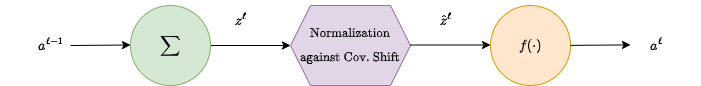
\includegraphics[width=100mm,scale=0.5]{images/nn_2_images/cov_shift_neuron.png}
                
                \caption*{Normalization/standardization can be treated just like any other module.}
            \end{figure}

            \phantom{}

            Note that this preserves the \orgg{information} in our input data:
            
            \begin{itemize}
                \item If one data point has one feature much larger than another, you'll still see that: the gap will just be shifted over to zero, and normalized.
                
            \end{itemize}

            \miniex Suppose you have some data: $[1,2,\red{100},3,4,5]$. If you standardize, you get

            \begin{equation}
                [-0.458, -0.433, \red{2.04}, -0.408, -0.383, -0.358, ]
            \end{equation}

            The larger data point still stands out above the rest!
            
            We need to be careful of dimensions:\\

            \begin{clarification}
                Normalization relies on the distribution (mean, s.d.) of our \purp{mini-batch}.

                But that means we can't just compute one data point at a time: we need to include the whole mini-batch of $k$ \gren{at the same time}.

                So, we have to change the dimensions of $Z^\ell$.

                $k$ is our \purp{batch size}, while $n$ is the number of \gren{dimensions}. 
                

                \begin{itemize}
                    \item $Z^\ell$ without norm: $(n^\ell \times 1)$
                    \item $Z^\ell$ with norm: $(n^\ell \times \red{k})$
                \end{itemize}

                We use $Z_{ij}^\ell$ to indicate the $\nth{i}$ dimension of the $\nth{j}$ data point.
            \end{clarification}
            

        

        \subsubsection{Post-Normalization: Choose Mean and S.D.}

            Now, we've adjusted it so that our distribution doesn't "drift", based on our training.

            But, now, we've \textbf{restricted} our model:
            
            \begin{itemize}
                \item We don't necessarily want our mean and standard deviation to be 0 and 1: it would be better to be able to \textbf{control} it.
            \end{itemize}
            
            To accomplish this, we'll \textbf{scale} and \textbf{shift} our input. Thus, we're choosing our mean/s.d. in a deliberate way.
            
            \begin{itemize}
                \item Each dimension needs its own mean and standard deviation.
                \item We have $n$ dimensions, and we need one variable to handle mean (or s.d.) for each: we'll need an $(n \times 1)$ vector.\\
            \end{itemize}

            \begin{concept}
                By doing \orgg{normalization}, we've transformed $Z$ into $\overline{Z}$. 
                
                \begin{itemize}
                    \item This "resets" our mean and standard deviation to 0 and 1.
                \end{itemize}

                However, we want to be able to \textbf{control} our mean and standard deviation. To do so, we introduce two new parameters:

                \begin{itemize}
                    \item $G$: An $(n \times 1)$ vector that \purp{scales} each of our dimensions $\overline{Z}_i$, giving our \purp{standard deviations}.
                    \item $B$: An $(n \times 1)$ vector that \gren{shifts} each of our dimensions $\overline{Z}_i$, giving our \gren{means}.
                \end{itemize}

                Thus, we get the true output of \vocab{batch normalization}:

                \begin{equation*}
                    \red{\widehat{Z}_{ik}} = \pur{G_i} * \red{\overline{Z}_{ij}} + \grn{B_i}
                \end{equation*}

            \end{concept}

            \miniex Here's a sample example using a vector $\overline{z}_j$: only considering one, post-normalization data point $j$. 

            \begin{equation}
                \begin{bmatrix}
                    \widehat{Z}_{1j} \\  \widehat{Z}_{2j} \\ \vdots \\ \widehat{Z}_{kj}
                \end{bmatrix}
                =
                \begin{bmatrix}
                    G_{1} \\  G_{2} \\ \vdots \\ G_{k}
                \end{bmatrix}
                *
                \begin{bmatrix}
                    \overline{Z}_{1j} \\  \overline{Z}_{2j} \\ \vdots \\ \overline{Z}_{kj}
                \end{bmatrix}
                +
                \begin{bmatrix}
                    B_{1} \\  B_{2} \\ \vdots \\ B_{k}
                \end{bmatrix}
            \end{equation}

            Where $*$ indicates element-wise multiplication.

            If we include this in our neuron graph, we now have two new modules:

            \begin{figure}[H]
                \centering
                    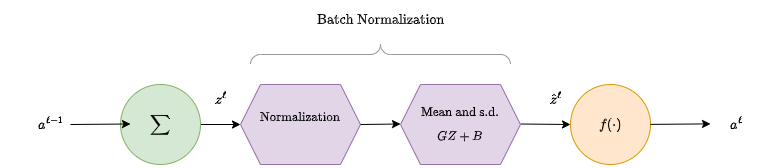
\includegraphics[width=120mm,scale=0.5]{images/nn_2_images/batch_normalization.png}
            \end{figure}

            \subsubsection{Full definition}


            \begin{definition}
                \vocab{Batch Normalization} is a process where we

                \begin{itemize}
                    \item Standardize the pre-activation for each layer using the mean $\mu_i$ and standard deviation $\sigma_i$ (for the $\nth{i}$ dimension). Select $\epsilon$: $0 < \epsilon<<1$.

                    \begin{equation*}
                        \red{ \overline{Z}_{ij} } =  \frac{ \red{Z_{ij}}  -\blu{\mu_i}}{\sigma_i+\epsilon}
                    \end{equation*}
                    
                    \item Choose the new mean and standard deviation for the pre-activation using $(n \times 1)$ vectors $G$ and $B$

                    \begin{equation*}
                        \red{\widehat{Z}_{ik}} = \pur{G_i} * \red{\overline{Z}_{ij}} + \grn{B_i}
                    \end{equation*}
                \end{itemize}
                
            \end{definition}

            \phantom{}

            \begin{concept}
                \vocab{Batch Normalization} is meant to accomplish the following:

                \begin{itemize}
                    \item Remove possible \purp{internal covariance shift}: training earlier layers may change the scale of inputs to later layers.
                        \begin{itemize}
                            \item This could make training more difficult.
                        \end{itemize}
                    \item Allow our model to \gren{select} a particular mean and s.d. for its pre-activation values, rather than arriving at them by chance.
                \end{itemize}

                It also tends to have a regularizing effect, and, in some learning algorithms, has replaced dropout.
            \end{concept}

        \subsubsection{Effectively Perturbs Data}

            We're not actually sure why normalization helps our models train. We originally designed it for \textbf{internal covariate shift}, but we're not sure if that's really \textbf{why} it works.

            One explanation might be that, due to random sampling, each mini-batch ends up slightly \textbf{modified} by our normalization.
            
            \begin{itemize}
                \item Since each batch is likely to have a slightly different mean/standard deviation, each one ends up differently "perturbed" by normalization.
            \end{itemize}

        \subsubsection{Applying batch normalization to backprop}

            We defer discussion of backprop to Appendix B.

    \pagebreak


\pagebreak
\section{Terms}
    \subsection*{Section 7-1}

    \begin{itemize}
        \item Neuron (Unit, Node)
        \item Neural Network
        \item Series and Parallel
        \item Linear Component
        \item Weight $w$
        \item Offset (Bias, Threshold) $w_0$
        \item Activation Function $f$
        \item Pre-activation $z$
        \item Activation $a$
        \item Identity Function
        \item Acyclic Networks
        \item Feed-forward Networks
        \item Layer
        \item Fully Connected
        \item Input dimension $m$
        \item Output dimension $n$
        \item Weight Matrix
        \item Offset Matrix
        \item Layer Notation $A^\ell$
        \item Step function
        \item ReLU function
        \item Sigmoid function
        \item Hyperbolic tangent function
        \item Softmax function
    \end{itemize}

    \subsection*{Section 7-2}

    
    \begin{itemize}
        \item Forward pass
        \item Back-Propagation
        \item Weight gradient
        \item Matrix Derivative
        \item Partial Derivative
        \item Multivariable Chain Rule
        \item Total Derivative
        \item Size of a matrix
        \item Planar Approximation
        \item Scalar/scalar derivative
        \item Vector/scalar derivative
        \item Scalar/vector derivative
        \item Vector/vector derivative
        \item Mini-batch
        \item Vanishing/Exploding Gradient
        \item Momentum (Optional)
        \item Adadelta (Optional)
        \item Adagrad (Optional)
        \item Adam (Optional)
        \item Normalization
        \item Early stopping (Review)
        \item Weight Decay
        \item Perturbation
        \item Dropout
        \item Covariate Shift
        \item Internal Covariate Shift
        \item Batch Normalization
        \item Multivariable Chain Rule (Review)
    \end{itemize}

